\documentclass[11pt,a4paper]{article}
\PassOptionsToPackage{hyphens}{url}
\usepackage[T1]{fontenc}
\usepackage[utf8]{inputenc}
\usepackage{tikz,pgfplots,booktabs,longtable,tabularx,siunitx,hyperref,geometry,xcolor,fancyhdr,caption,amsmath}
\usetikzlibrary{arrows.meta,positioning,calc}
\pgfplotsset{compat=1.18,every axis/.append style={tick label style={font=\small},label style={font=\small},legend style={font=\footnotesize,draw=none},grid=major,grid style={gray!15}}}
\geometry{margin=22mm,headheight=15pt}
\definecolor{ink}{HTML}{173D3D}\definecolor{teal}{HTML}{267C78}\definecolor{gold}{HTML}{C18B2E}\definecolor{red}{HTML}{A84238}
\hypersetup{colorlinks=true,linkcolor=teal,citecolor=teal,urlcolor=teal,pdftitle={ZeroWatt Wind - Evidence and Feasibility}}
\urlstyle{same}\Urlmuskip=0mu plus 1mu\relax\setlength{\emergencystretch}{3em}\setlength{\parskip}{5pt}\setlength{\parindent}{0pt}
\sisetup{group-separator={,},group-minimum-digits=4,detect-all}
\pagestyle{fancy}\fancyhf{}\fancyhead[L]{\small\textcolor{ink}{ZeroWatt Wind}}\fancyhead[R]{\small Feasibility and business evidence}\fancyfoot[C]{\thepage}
\captionsetup{font=small,labelfont=bf}\setcounter{tocdepth}{1}
\begin{document}
\begin{titlepage}
\vspace*{1.4cm}
{\color{teal}\large RESEARCH AND INVESTMENT SCREENING}\par\vspace{.5cm}
{\Huge\bfseries\color{ink}ZeroWatt Wind}\par\vspace{.5cm}
{\LARGE Evidence-backed feasibility\\and business report}\par\vspace{1cm}
\rule{\linewidth}{1pt}\par
Wind-driven mechanical ventilation and supplemental pond aeration in Bangladesh\par\vspace{.6cm}
{\large Decision: fund a gated validation pilot; commercial rollout is not yet supported.}\par\vspace{1cm}
Prepared for renewable-energy judges, investors and university evaluators.\par
Research cut-off: 22 October 2026 (Asia/Dhaka).\par
Baseline: supplied project submission, poster and audited repository source.\par\vfill
\textbf{Reading the evidence.} [S] is an attributed observation or published value; [D] is a reproducible calculation; [A] is an explicit scenario assumption. A source that describes a prototype does not validate its output. Low, base and high allowances are not supplier quotations. Values marked NOT FOUND remain unresolved. All figures are vector drawings embedded in this single file.\par
\end{titlepage}
\section*{Executive summary}\addcontentsline{toc}{section}{Executive summary}
\textbf{Verdict.} The printed prototype demonstrates a mechanical idea, while the poster expressly leaves airflow, starting wind speed, torque, drivetrain loss and oxygen transfer unmeasured. \cite{poster,project} The business should purchase evidence before purchasing scale. A limited, supervised supplemental-use pilot is defensible; a claim of guaranteed clinical ventilation or fish-survival protection is not.

{\small
\setlength{\tabcolsep}{3pt}\renewcommand{\arraystretch}{1.18}
\begin{longtable}{@{}>{\raggedright\arraybackslash}p{0.3033\linewidth}>{\raggedright\arraybackslash}p{0.3033\linewidth}>{\raggedright\arraybackslash}p{0.3033\linewidth}@{}}
\toprule \textbf{Base case headline} & \textbf{Result} & \textbf{Basis} \\ \midrule
\endfirsthead\toprule \textbf{Base case headline} & \textbf{Result} & \textbf{Basis} \\ \midrule
\endhead\bottomrule\endfoot
Project NPV, nominal BDT & \num{-11181078} & [D] monthly FCF, assumed required return \\
Project NPV, USD equivalent & \num{-90425} & [D] dated conversion \\
Annual effective project IRR & \num{-47.7}\% & [D] negative; unique bracketed root \\
Simple / discounted payback & Not reached within model horizon & [D] cumulative cash flow remains negative \\
Initial investment / peak cumulative funding need & \num{2240000} / \num{21769906} & [D] no grant or exit-value rescue \\
Basic A / pond B / combined A+B ex-works BOM & \num{40000} / \num{43200} / \num{83200} & [D] from [A] production allowances \\
\end{longtable}}
The base screening assumes a site mean wind of \num{3.5} [A] m/s. It predicts full additional-flow performance for \num{29.2}\% [D] of time after mechanical availability, distinct from an energy displacement fraction of \num{47.1}\% [D]. These probabilities come from an assumed distribution, not a Bangladesh rooftop measurement.

The NPV discount rate is \num{18}\% [A], tested alongside \num{12}\% [A] and \num{25}\% [A]. The historical Bangladesh Bank policy benchmark was \num{10}\% [S]; the project risk premium is an analyst assumption. \cite{rate}

Commercial tariffs, willingness to pay, adoption, component quotations and durability remain weakly evidenced. The optimistic scenario is conditional and profitable; it is not a probability-weighted forecast. Currency: \num{123.65} [S] BDT/USD, Bangladesh Bank weighted average dated 2026-10-19, accessed 2026-10-22. \cite{fx}

\clearpage\tableofcontents
\clearpage\section{Problem sizing and the addressable need}
Poor indoor air and pond oxygen matter, but their national consequences must not be attributed wholesale to this device. World Bank estimates combine outdoor and household pollution, unsafe water, sanitation and lead; they are not a ventilation-only loss estimate. \cite{wb}

{\small
\setlength{\tabcolsep}{3pt}\renewcommand{\arraystretch}{1.18}
\begin{longtable}{@{}>{\raggedright\arraybackslash}p{0.2730\linewidth}>{\raggedright\arraybackslash}p{0.2730\linewidth}>{\raggedright\arraybackslash}p{0.3640\linewidth}@{}}
\toprule \textbf{Evidence / boundary} & \textbf{Value} & \textbf{Basis} \\ \midrule
\endfirsthead\toprule \textbf{Evidence / boundary} & \textbf{Value} & \textbf{Basis} \\ \midrule
\endhead\bottomrule\endfoot
National pond area & \num{424168} ha & [S] DoF, reporting period 2023-24 \cite{dof} \\
Number of ponds & \num{2543869} & [S] DoF table on culture intensity; not paying customers \cite{dof} \\
Annual pond fish production & \num{2368741} tonnes & [S] DoF \cite{dof} \\
National combined pollution burden & Over \num{272000} premature deaths; \num{5200000000} illness days/year & [S] Context only \cite{wb} \\
Household and outdoor air pollution health cost & \num{8.32}\% of GDP (2019) & [S] Historical national burden \cite{wb} \\
\end{longtable}}
The project repeats a claim linking \num{500} [S] ppm additional CO2 with a \num{15} [S]\% cognitive-performance reduction. The institutional description and primary-study record concern specific observational test endpoints. A general causal productivity loss at this exact percentage was NOT VERIFIED and is excluded from revenue, health savings and NPV. \cite{poster,harvard,cognition}

FAO describes oxygen depletion and reduced growth in Bangladesh ponds, including warm calm nights and cloudy monsoon conditions. A Bangladesh heatwave report corroborates the mechanism but does not quantify national losses attributable only to low DO. These sources do not establish this prototype prevents fish kills. \cite{fao,heatnews}

\subsection{A site-level loss exposure, not an avoided-loss promise}
An illustrative \num{1000} [A] kg stock at \num{200} [A] BDT/kg and a \num{10}\% [A] event loss exposes \num{20000} [D] BDT. Low/high loss fractions are \num{2}\% [A] / \num{30}\% [A]. The event probability and avoidable fraction are NOT FOUND; no expected-value benefit is booked. Time spent manually splashing, fetching fuel or servicing the unit is likewise NOT FOUND; travel/labour allowances are in OPEX.

Using the illustrative room duty, clinic electricity costs \num{2180} [D] BDT/year before fixed fees and taxes. This modest energy bill constrains an energy-only product price. Load-shedding coincidence with useful wind is NOT FOUND. Neither a mortality-reduction total nor a fish-yield uplift is fabricated.

\clearpage\section{Solution, engineering boundary and simulation audit}
The mechanical core captures wind with a spiral rotor and transmits rotation through shafts and bevel gears to either a fan or paddles. The combined physical case in this report is a separate roof installation plus a separate pond installation; their energy is not counted twice. The advanced website adds PV, battery, motor, controls and freewheels; it is not an electricity-free extension. \cite{poster,project,site}

\begin{figure}[htbp]\centering
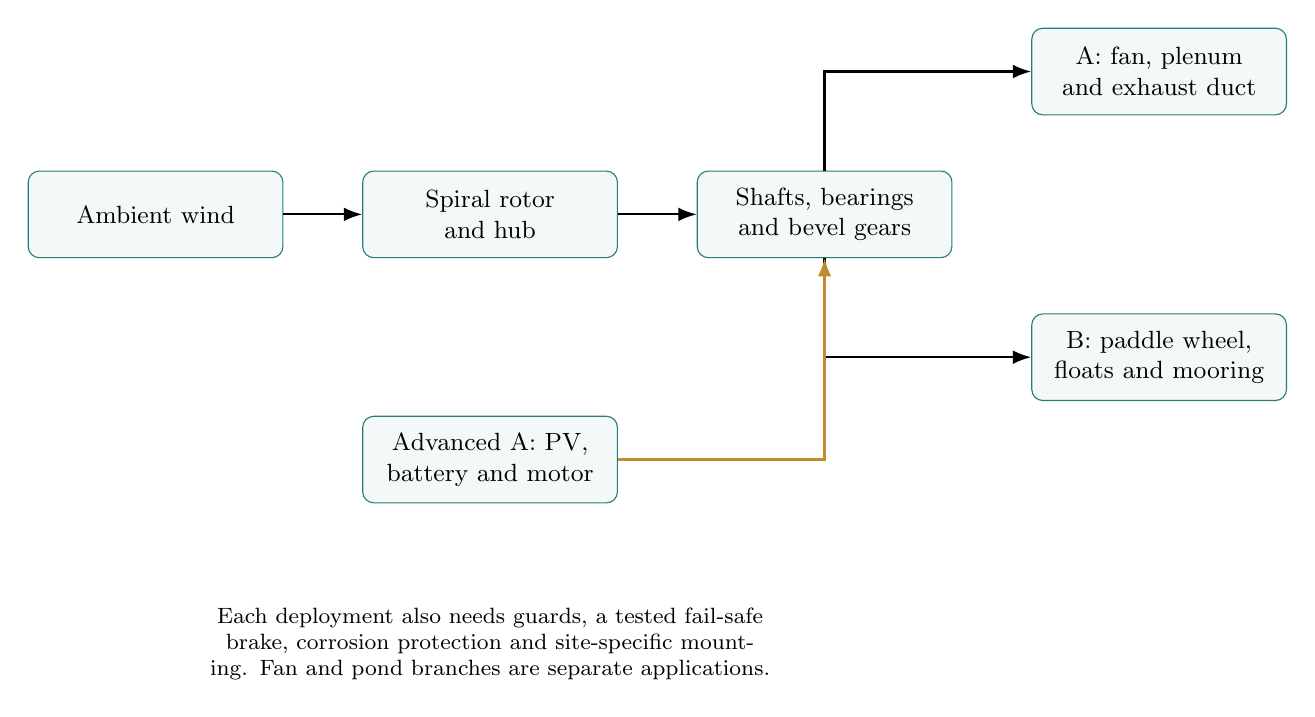
\begin{tikzpicture}[node distance=7mm and 10mm,box/.style={draw=teal,rounded corners,fill=teal!5,align=center,text width=30mm,minimum height=11mm,font=\small},>=Latex]
\node[box] (wind) {Ambient wind};\node[box,right=of wind] (rotor) {Spiral rotor\\and hub};\node[box,right=of rotor] (drive) {Shafts, bearings\\and bevel gears};
\node[box,above right=7mm and 10mm of drive] (fan) {A: fan, plenum\\and exhaust duct};
\node[box,below right=7mm and 10mm of drive] (pond) {B: paddle wheel,\\floats and mooring};
\draw[->,thick] (wind)--(rotor);\draw[->,thick] (rotor)--(drive);\draw[->,thick] (drive)|-(fan);\draw[->,thick] (drive)|-(pond);
\node[box,below=20mm of rotor] (pv) {Advanced A: PV,\\battery and motor};\draw[->,gold,thick] (pv)-|(drive);
\node[align=center,font=\footnotesize,text width=100mm,below=12mm of pv] {Each deployment also needs guards, a tested fail-safe brake, corrosion protection and site-specific mounting. Fan and pond branches are separate applications.};
\end{tikzpicture}\caption{System pathways [S] project concept, with [A] production protection and advanced assistance boundary.}\end{figure}
\subsection{What the code computes}
For the basic geometry, $P_s=\min(\tfrac12\rho A v^3C_p\eta_d,P_r)$ above the assumed starting speed; $Q=P_s\eta_f\,3600/\Delta p$. The room model is a perfectly mixed equilibrium CO2 balance. The pond model applies standard oxygen transfer, a temperature/saturation correction, background reaeration and constant oxygen demand. It does not integrate a whole-night oxygen budget. \cite{site}

{\small
\setlength{\tabcolsep}{3pt}\renewcommand{\arraystretch}{1.18}
\begin{longtable}{@{}>{\raggedright\arraybackslash}p{0.2022\linewidth}>{\raggedright\arraybackslash}p{0.2612\linewidth}>{\raggedright\arraybackslash}p{0.2612\linewidth}>{\raggedright\arraybackslash}p{0.1854\linewidth}@{}}
\toprule \textbf{Parameter} & \textbf{Basic / pond default} & \textbf{Advanced default} & \textbf{Basis} \\ \midrule
\endfirsthead\toprule \textbf{Parameter} & \textbf{Basic / pond default} & \textbf{Advanced default} & \textbf{Basis} \\ \midrule
\endhead\bottomrule\endfoot
Swept rotor size & \num{1.0} m diameter & \num{3.46} m$^2$ area & [A] Different geometries \\
Power coefficient / drivetrain efficiency & \num{0.18} / \num{0.75} & \num{0.23} / \num{0.84} & [A] Untested coefficients \\
Fan model & \num{20} Pa; \num{0.35} efficiency & \num{60} W at \num{240} RPM & [A] Not a certified curve \\
Room / pond volume & \num{150} / \num{100} m$^3$ & Same scene; separate model & [A] Default sizes \\
CO2 / DO targets & \num{1200} ppm / \num{4} mg/L & No clinical certification & [A] Demo targets \\
Pond standard SAE / demand & \num{0.80} kg/kWh; \num{0.25} mg/L/h & Not implemented & [A] Transfer model \\
PV / battery / motor & None for uninstrumented core & \num{180} W / \num{240} Wh / \num{95} W input & [A] Site concept \\
Battery lock / recovery & No battery & \num{12}\% / \num{20}\% & [A] Control thresholds \\
Assistance on/off / verification & No motor & \num{0.90} / \num{1.05} target; \num{1.5} s & [A] Hysteresis \\
\end{longtable}}
\subsection{Every weather case and operating demonstration}
{\small
\setlength{\tabcolsep}{3pt}\renewcommand{\arraystretch}{1.18}
\begin{longtable}{@{}>{\raggedright\arraybackslash}p{0.1114\linewidth}>{\raggedright\arraybackslash}p{0.1671\linewidth}>{\raggedright\arraybackslash}p{0.1857\linewidth}>{\raggedright\arraybackslash}p{0.3436\linewidth}>{\raggedright\arraybackslash}p{0.1021\linewidth}@{}}
\toprule \textbf{Mode} & \textbf{Case} & \textbf{Wind / pattern} & \textbf{What it does not establish} & \textbf{Basis} \\ \midrule
\endfirsthead\toprule \textbf{Mode} & \textbf{Case} & \textbf{Wind / pattern} & \textbf{What it does not establish} & \textbf{Basis} \\ \midrule
\endhead\bottomrule\endfoot
Basic A & Rooftop breeze & \num{4.5} m/s; steady & Steady illustrative operation; no measured power curve. & [A] \cite{site} \\
Basic A & Urban canyon & \num{2.8} m/s; lull & Shelter/lulls; no urban turbulence or fatigue validation. & [A] \cite{site} \\
Basic A & Heatwave & \num{2.3} m/s; gusts & Heat exposure warnings; no refrigeration or humidity guarantee. & [A] \cite{site} \\
Basic A & Monsoon & \num{7.0} m/s; gusts & Rain effects and optional damper; not waterproof certification. & [A] \cite{site} \\
Basic A & Cyclone & \num{19.0} m/s; storm & Display continues spinning; no automatic safe cut-out. & [A] \cite{site} \\
Pond B & Park breeze & \num{4.5} m/s; steady & Steady illustrative operation; no measured power curve. & [A] \cite{site} \\
Pond B & Sheltered lull & \num{2.8} m/s; lull & Repeating lull is synthetic, not a weather time series. & [A] \cite{site} \\
Pond B & Hot night & \num{2.2} m/s; gusts & Pre-dawn oxygen risk; no survival or transient DO proof. & [A] \cite{site} \\
Pond B & Monsoon & \num{7.0} m/s; gusts & Rain effects and optional damper; not waterproof certification. & [A] \cite{site} \\
Pond B & Storm surge & \num{19.0} m/s; storm & Display continues spinning; no automatic safe cut-out. & [A] \cite{site} \\
\end{longtable}}
{\small
\setlength{\tabcolsep}{3pt}\renewcommand{\arraystretch}{1.18}
\begin{longtable}{@{}>{\raggedright\arraybackslash}p{0.1963\linewidth}>{\raggedright\arraybackslash}p{0.3123\linewidth}>{\raggedright\arraybackslash}p{0.3123\linewidth}>{\raggedright\arraybackslash}p{0.0892\linewidth}@{}}
\toprule \textbf{Advanced control / state} & \textbf{Demonstration} & \textbf{Limit} & \textbf{Basis} \\ \midrule
\endfirsthead\toprule \textbf{Advanced control / state} & \textbf{Demonstration} & \textbf{Limit} & \textbf{Basis} \\ \midrule
\endhead\bottomrule\endfoot
Sunny / sun position & PV drives or charges while the illustrated tracker follows sun position. & No measured tracking gain, shading or thermal model. & [A] \cite{site} \\
Canyon & Sheltered wind with solar assistance. & No site-specific solar/wind joint distribution. & [A] \\
Monsoon & PV and motor assistance are disabled by policy. & Physical PV is not inherently zero in every overcast condition. & [A] \\
Adequate / weak / no wind & Wind-only, shared torque, or motor-driven fan through freewheels. & No clutch durability or measured torque curve. & [A] \\
Low battery / night & Hysteretic motor lockout; battery drains with no PV at night. & Short autonomy; no guaranteed night service. & [A] \\
Injected fault / wind-only & Motor inhibited, mechanical wind path remains. & No certified functional-safety system. & [A] \\
Pause / speed / section / explode / tour & Presentation and inspection controls; exploded flow paths hidden. & No fabrication geometry or independent engineering proof. & [A] \\
Moving / moored pond boats & Changes visual mounting and unit count. & No mooring loads, navigation, capsize or hydrodynamic validation. & [A] \\
\end{longtable}}
Wind profile selectors include steady, gusts, repeating lull and storm. Hardware choices cover cup/ultrasonic or Hall wind sensing; MQ-135, MH-Z19B, SCD41 or industrial CO2; analog/galvanic/optical DO; rain and water-temperature probes; ATtiny, Uno, Pico, ESP32 or STM32; and open, IP54 or IP67 enclosures. The code applies temperature, ingress and power assumptions. Sensor ratings are not verified datasheets. Electronics require an external power supply, and warnings do not replace a mechanical brake. A complete literal/parameter inventory is retained in the repository audit. \cite{site}

At the basic rooftop breeze preset, the code gives \num{5.92} [D] W and \num{372.8} [D] m$^3$/h, or \num{2.49} [D] added ACH. These are calculated examples, not measurements. The advanced rated-flow assumption yields \num{5.67} [D] added ACH. The illustrative battery from its default charge to lockout supplies only \num{1.87} [D] hours at nominal motor demand without wind, PV or parasitic loads.

Older naturally ventilated clinic guidance discussed in the clinic study implies \num{1728} [D] m$^3$/h for the default occupancy. The financial example below targets a smaller incremental flow; it cannot be represented as compliance with that guidance. Real intake pollution, thermal comfort, filtration pressure loss and room mixing require assessment. \cite{clinic,whoweb}

\clearpage\section{Components, market evidence and production costs}
The baseline prototype uses PLA, but a production candidate uses supported metal shafts/gears, protected structure and inspectable floats. Proposed dimensions and quantities are design assumptions pending stress, thermal and water tests. Catalogue gear selection depends on module, ratio, material, bore and permitted loads; a cheap model gear is not an equivalent part. \cite{project,khk,windguide}

\subsection{Observed prices and the three-quote test}
{\footnotesize
\setlength{\tabcolsep}{3pt}\renewcommand{\arraystretch}{1.18}
\begin{longtable}{@{}>{\raggedright\arraybackslash}p{0.2650\linewidth}>{\raggedright\arraybackslash}p{0.1414\linewidth}>{\raggedright\arraybackslash}p{0.1944\linewidth}>{\raggedright\arraybackslash}p{0.3092\linewidth}@{}}
\toprule \textbf{Family / supplier} & \textbf{Visible price} & \textbf{BDT / USD} & \textbf{Caveat and basis} \\ \midrule
\endfirsthead\toprule \textbf{Family / supplier} & \textbf{Visible price} & \textbf{BDT / USD} & \textbf{Caveat and basis} \\ \midrule
\endhead\bottomrule\endfoot
PLA filament kg / HTE Bangladesh & \num{1287.00} BDT & \num{1287.00} / \num{10.41} & open text; out of stock on recheck; [S] indication, [D] FX \cite{filament3} \\
PLA filament kg / Costareen & \num{1550.00} BDT & \num{1550.00} / \num{12.54} & dated guide starting price; [S] indication, [D] FX \cite{filament1} \\
PLA filament kg / Electronics.Com.BD & \num{1999.00} BDT & \num{1999.00} / \num{16.17} & open text; [S] indication, [D] FX \cite{filament4} \\
PLA filament kg / TechShopBD & \num{1950.04} BDT & \num{1950.04} / \num{15.77} & open marketplace; [S] indication, [D] FX \cite{filament2} \\
UCP204 bearing / Daraz/Fair Enterprise & \num{450.00} BDT & \num{450.00} / \num{3.64} & cached stock conflicting; [S] indication, [D] FX \cite{bearing1} \\
UCP204 bearing / MISUMI & \num{15.65} SGD & \num{1511.56} / \num{12.22} & search-index only; open 429; [S] indication, [D] FX \cite{bearing2} \\
UCP204 bearing / Motion & \num{52.70} USD & \num{6516.36} / \num{52.70} & open text; [S] indication, [D] FX \cite{bearing3} \\
Electric exhaust fan / Walton & \num{1250.00} BDT & \num{1250.00} / \num{10.11} & open full text; index showed 1310; [S] indication, [D] FX \cite{fanweb} \\
Hobby bevel gear / ZerOneTech & \num{245.00} BDT & \num{245.00} / \num{1.98} & search-index only; open failed; [S] indication, [D] FX \cite{gear} \\
Conventional aerator / NSC BD & \num{50000.00} BDT & \num{50000.00} / \num{404.37} & open text; [S] indication, [D] FX \cite{aerator1} \\
Conventional aerator / Bangla Ltd. & \num{40000.00} BDT & \num{40000.00} / \num{323.49} & open text; inconsistent transfer claims; [S] indication, [D] FX \cite{banglaaer} \\
Conventional aerator / BDStall single seller & \num{40000.00} BDT & \num{40000.00} / \num{323.49} & open text; seller independence not established; [S] indication, [D] FX \cite{bdstall} \\
Battery 12V20Ah / CityTechBD & \num{1845.00} BDT & \num{1845.00} / \num{14.92} & open text; suspicious outlier; [S] indication, [D] FX \cite{battery1} \\
Battery 12V20Ah / Teexla & \num{8200.00} BDT & \num{8200.00} / \num{66.32} & open text; [S] indication, [D] FX \cite{battery2} \\
\end{longtable}}
Prices were observed on 2026-10-22. Listings without publication dates are undated; stock and cached prices can differ. The Walton full page displayed a lower price than its indexed result; the opened full-page price is used. Foreign prices are not landed Bangladesh quotes. MISUMI and the hobby-gear price remain index-only and low-confidence. The low battery listing is an outlier and is excluded from the warranted production battery allowance.

{\small
\setlength{\tabcolsep}{3pt}\renewcommand{\arraystretch}{1.18}
\begin{longtable}{@{}>{\raggedright\arraybackslash}p{0.2209\linewidth}>{\raggedright\arraybackslash}p{0.0883\linewidth}>{\raggedright\arraybackslash}p{0.2827\linewidth}>{\raggedright\arraybackslash}p{0.3181\linewidth}@{}}
\toprule \textbf{Family} & \textbf{Seller count} & \textbf{Low / median / high BDT} & \textbf{Basis / limitation} \\ \midrule
\endfirsthead\toprule \textbf{Family} & \textbf{Seller count} & \textbf{Low / median / high BDT} & \textbf{Basis / limitation} \\ \midrule
\endhead\bottomrule\endfoot
Battery 12V20Ah & \num{2} & \num{1845.00} / \num{5022.50} / \num{8200.00} & Three comparable independent landed quotes NOT FOUND; [D] indication summary \\
Conventional aerator & \num{2} & \num{40000.00} / \num{40000.00} / \num{50000.00} & Three comparable independent landed quotes NOT FOUND; [D] indication summary \\
Electric exhaust fan & \num{1} & \num{1250.00} / \num{1250.00} / \num{1250.00} & Three comparable independent landed quotes NOT FOUND; [D] indication summary \\
Hobby bevel gear & \num{1} & \num{245.00} / \num{245.00} / \num{245.00} & Three comparable independent landed quotes NOT FOUND; [D] indication summary \\
PLA filament kg & \num{4} & \num{1287.00} / \num{1750.02} / \num{1999.00} & Family-level comparison only; brands differ; [D] indication summary \\
UCP204 bearing & \num{3} & \num{450.00} / \num{1511.56} / \num{6516.36} & Three comparable independent landed quotes NOT FOUND; [D] indication summary \\
\end{longtable}}
Only filament has multiple independent, broadly comparable local price observations. Generic and branded bearing grades differ. Three current, independent production quotations for each bespoke component are NOT FOUND. The BOM low/base/high columns below are allowances [A], not a substituted quotation median. Supplier statements about oxygen output also differ internally; they are not accepted as field SAE. \cite{banglaaer,faoaer}

\subsection{Costed production BOM for each application}
\subsection{A: basic rooftop ventilation}
{\footnotesize
\setlength{\tabcolsep}{3pt}\renewcommand{\arraystretch}{1.18}
\begin{longtable}{@{}>{\raggedright\arraybackslash}p{0.3784\linewidth}>{\raggedright\arraybackslash}p{0.0541\linewidth}>{\raggedright\arraybackslash}p{0.2613\linewidth}>{\raggedright\arraybackslash}p{0.2162\linewidth}@{}}
\toprule \textbf{Component, material/specification} & \textbf{Qty} & \textbf{Low / base / high BDT} & \textbf{Function / basis} \\ \midrule
\endfirsthead\toprule \textbf{Component, material/specification} & \textbf{Qty} & \textbf{Low / base / high BDT} & \textbf{Function / basis} \\ \midrule
\endhead\bottomrule\endfoot
Spiral rotor and balanced hub. Formed aluminium; 1 m nominal basic / 2.1 m hybrid & \num{1} & \num{3500} / \num{6000} / \num{10000} & Capture wind; [A], production quotes NOT FOUND \\
Shaft stock and machining. Steel, nominal 20 mm; three axes for two stages, two for H & \num{3} & \num{1500} / \num{2700} / \num{4800} & Transmit torque; [A], production quotes NOT FOUND \\
Production bevel gear pair. Steel, two right-angle stages; module and rating RFQ & \num{2} & \num{1400} / \num{3000} / \num{6000} & Redirect rotation; [A], production quotes NOT FOUND \\
Radial bearing blocks. 20 mm sealed UCP-type; two radial supports per shaft; axial separate & \num{6} & \num{2700} / \num{5400} / \num{12000} & Support shaft; [A], production quotes NOT FOUND \\
Thrust bearing and collar set. Matched axial load and positive retention & \num{1} & \num{500} / \num{1000} / \num{2000} & Carry fan/gear thrust; [A], production quotes NOT FOUND \\
Couplings keys collars. Keyed steel; fastener locking & \num{3} & \num{600} / \num{1200} / \num{2100} & Locate and couple shafts; [A], production quotes NOT FOUND \\
Frame mounting and isolators. Coated local steel; engineered anchor plates & \num{1} & \num{2500} / \num{4500} / \num{7500} & Structural support; [A], production quotes NOT FOUND \\
Fail-safe brake and storm restraint. Mechanical brake/furling concept; test required & \num{1} & \num{1000} / \num{2500} / \num{5000} & Overspeed protection; [A], production quotes NOT FOUND \\
Rotor and gear guards. Corrosion-resistant mesh with access covers & \num{1} & \num{1000} / \num{1800} / \num{3500} & Entanglement protection; [A], production quotes NOT FOUND \\
Seals grease fasteners coating. Gaskets, compatible lubricant, corrosion isolation & \num{1} & \num{700} / \num{1200} / \num{2200} & Weather and service kit; [A], production quotes NOT FOUND \\
Mechanical axial fan and hub. NACA 65-810 concept; needs pressure-flow test & \num{1} & \num{1200} / \num{2200} / \num{4000} & Exhaust room air; [A], production quotes NOT FOUND \\
Sleeve plenum duct and cowl. Sheet metal; screened intake, access and rain drain & \num{1} & \num{1800} / \num{3500} / \num{6500} & Air pathway; [A], production quotes NOT FOUND \\
Roof flashing and backdraft damper. Waterproof penetration and service access & \num{1} & \num{800} / \num{1500} / \num{3000} & Weatherproof building interface; [A], production quotes NOT FOUND \\
Assembly balancing and inspection. Paid shop labour and acceptance test & \num{1} & \num{2000} / \num{3500} / \num{6000} & Deliver inspected ex-works unit; [A], production quotes NOT FOUND \\
\end{longtable}}
\subsection{B: pond aeration}
{\footnotesize
\setlength{\tabcolsep}{3pt}\renewcommand{\arraystretch}{1.18}
\begin{longtable}{@{}>{\raggedright\arraybackslash}p{0.3784\linewidth}>{\raggedright\arraybackslash}p{0.0541\linewidth}>{\raggedright\arraybackslash}p{0.2613\linewidth}>{\raggedright\arraybackslash}p{0.2162\linewidth}@{}}
\toprule \textbf{Component, material/specification} & \textbf{Qty} & \textbf{Low / base / high BDT} & \textbf{Function / basis} \\ \midrule
\endfirsthead\toprule \textbf{Component, material/specification} & \textbf{Qty} & \textbf{Low / base / high BDT} & \textbf{Function / basis} \\ \midrule
\endhead\bottomrule\endfoot
Spiral rotor and balanced hub. Formed aluminium; 1 m nominal basic / 2.1 m hybrid & \num{1} & \num{3500} / \num{6000} / \num{10000} & Capture wind; [A], production quotes NOT FOUND \\
Shaft stock and machining. Steel, nominal 20 mm; three axes for two stages, two for H & \num{3} & \num{1500} / \num{2700} / \num{4800} & Transmit torque; [A], production quotes NOT FOUND \\
Production bevel gear pair. Steel, two right-angle stages; module and rating RFQ & \num{2} & \num{1400} / \num{3000} / \num{6000} & Redirect rotation; [A], production quotes NOT FOUND \\
Radial bearing blocks. 20 mm sealed UCP-type; two radial supports per shaft; axial separate & \num{6} & \num{2700} / \num{5400} / \num{12000} & Support shaft; [A], production quotes NOT FOUND \\
Thrust bearing and collar set. Matched axial load and positive retention & \num{1} & \num{500} / \num{1000} / \num{2000} & Carry fan/gear thrust; [A], production quotes NOT FOUND \\
Couplings keys collars. Keyed steel; fastener locking & \num{3} & \num{600} / \num{1200} / \num{2100} & Locate and couple shafts; [A], production quotes NOT FOUND \\
Frame mounting and isolators. Coated local steel; engineered anchor plates & \num{1} & \num{2500} / \num{4500} / \num{7500} & Structural support; [A], production quotes NOT FOUND \\
Fail-safe brake and storm restraint. Mechanical brake/furling concept; test required & \num{1} & \num{1000} / \num{2500} / \num{5000} & Overspeed protection; [A], production quotes NOT FOUND \\
Rotor and gear guards. Corrosion-resistant mesh with access covers & \num{1} & \num{1000} / \num{1800} / \num{3500} & Entanglement protection; [A], production quotes NOT FOUND \\
Seals grease fasteners coating. Gaskets, compatible lubricant, corrosion isolation & \num{1} & \num{700} / \num{1200} / \num{2200} & Weather and service kit; [A], production quotes NOT FOUND \\
Paddle wheel and wet shaft guards. HDPE paddles on corrosion-resistant hub & \num{1} & \num{1800} / \num{3500} / \num{6000} & Surface aeration; [A], production quotes NOT FOUND \\
Compartmented pontoons. Recovered/rotomoulded HDPE, two separate floats & \num{2} & \num{2400} / \num{4400} / \num{8000} & Flotation with reserve buoyancy; [A], production quotes NOT FOUND \\
Mooring anchor retrieval and wet seals. Two lines, anchors and dry access provision & \num{1} & \num{1200} / \num{2500} / \num{5000} & Retain and retrieve pond assembly; [A], production quotes NOT FOUND \\
Assembly balancing and inspection. Paid shop labour and acceptance test & \num{1} & \num{2000} / \num{3500} / \num{6000} & Deliver inspected ex-works unit; [A], production quotes NOT FOUND \\
\end{longtable}}
\subsection{Combined A+B: two separate installed assemblies}
{\footnotesize
\setlength{\tabcolsep}{3pt}\renewcommand{\arraystretch}{1.18}
\begin{longtable}{@{}>{\raggedright\arraybackslash}p{0.3784\linewidth}>{\raggedright\arraybackslash}p{0.0541\linewidth}>{\raggedright\arraybackslash}p{0.2613\linewidth}>{\raggedright\arraybackslash}p{0.2162\linewidth}@{}}
\toprule \textbf{Component, material/specification} & \textbf{Qty} & \textbf{Low / base / high BDT} & \textbf{Function / basis} \\ \midrule
\endfirsthead\toprule \textbf{Component, material/specification} & \textbf{Qty} & \textbf{Low / base / high BDT} & \textbf{Function / basis} \\ \midrule
\endhead\bottomrule\endfoot
Spiral rotor and balanced hub. Formed aluminium; 1 m nominal basic / 2.1 m hybrid & \num{2} & \num{7000} / \num{12000} / \num{20000} & Capture wind; [A], production quotes NOT FOUND \\
Shaft stock and machining. Steel, nominal 20 mm; three axes for two stages, two for H & \num{6} & \num{3000} / \num{5400} / \num{9600} & Transmit torque; [A], production quotes NOT FOUND \\
Production bevel gear pair. Steel, two right-angle stages; module and rating RFQ & \num{4} & \num{2800} / \num{6000} / \num{12000} & Redirect rotation; [A], production quotes NOT FOUND \\
Radial bearing blocks. 20 mm sealed UCP-type; two radial supports per shaft; axial separate & \num{12} & \num{5400} / \num{10800} / \num{24000} & Support shaft; [A], production quotes NOT FOUND \\
Thrust bearing and collar set. Matched axial load and positive retention & \num{2} & \num{1000} / \num{2000} / \num{4000} & Carry fan/gear thrust; [A], production quotes NOT FOUND \\
Couplings keys collars. Keyed steel; fastener locking & \num{6} & \num{1200} / \num{2400} / \num{4200} & Locate and couple shafts; [A], production quotes NOT FOUND \\
Frame mounting and isolators. Coated local steel; engineered anchor plates & \num{2} & \num{5000} / \num{9000} / \num{15000} & Structural support; [A], production quotes NOT FOUND \\
Fail-safe brake and storm restraint. Mechanical brake/furling concept; test required & \num{2} & \num{2000} / \num{5000} / \num{10000} & Overspeed protection; [A], production quotes NOT FOUND \\
Rotor and gear guards. Corrosion-resistant mesh with access covers & \num{2} & \num{2000} / \num{3600} / \num{7000} & Entanglement protection; [A], production quotes NOT FOUND \\
Seals grease fasteners coating. Gaskets, compatible lubricant, corrosion isolation & \num{2} & \num{1400} / \num{2400} / \num{4400} & Weather and service kit; [A], production quotes NOT FOUND \\
Mechanical axial fan and hub. NACA 65-810 concept; needs pressure-flow test & \num{1} & \num{1200} / \num{2200} / \num{4000} & Exhaust room air; [A], production quotes NOT FOUND \\
Sleeve plenum duct and cowl. Sheet metal; screened intake, access and rain drain & \num{1} & \num{1800} / \num{3500} / \num{6500} & Air pathway; [A], production quotes NOT FOUND \\
Roof flashing and backdraft damper. Waterproof penetration and service access & \num{1} & \num{800} / \num{1500} / \num{3000} & Weatherproof building interface; [A], production quotes NOT FOUND \\
Paddle wheel and wet shaft guards. HDPE paddles on corrosion-resistant hub & \num{1} & \num{1800} / \num{3500} / \num{6000} & Surface aeration; [A], production quotes NOT FOUND \\
Compartmented pontoons. Recovered/rotomoulded HDPE, two separate floats & \num{2} & \num{2400} / \num{4400} / \num{8000} & Flotation with reserve buoyancy; [A], production quotes NOT FOUND \\
Mooring anchor retrieval and wet seals. Two lines, anchors and dry access provision & \num{1} & \num{1200} / \num{2500} / \num{5000} & Retain and retrieve pond assembly; [A], production quotes NOT FOUND \\
Assembly balancing and inspection. Paid shop labour and acceptance test & \num{2} & \num{4000} / \num{7000} / \num{12000} & Deliver inspected ex-works unit; [A], production quotes NOT FOUND \\
\end{longtable}}
\subsection{H: advanced hybrid ventilation}
{\footnotesize
\setlength{\tabcolsep}{3pt}\renewcommand{\arraystretch}{1.18}
\begin{longtable}{@{}>{\raggedright\arraybackslash}p{0.3784\linewidth}>{\raggedright\arraybackslash}p{0.0541\linewidth}>{\raggedright\arraybackslash}p{0.2613\linewidth}>{\raggedright\arraybackslash}p{0.2162\linewidth}@{}}
\toprule \textbf{Component, material/specification} & \textbf{Qty} & \textbf{Low / base / high BDT} & \textbf{Function / basis} \\ \midrule
\endfirsthead\toprule \textbf{Component, material/specification} & \textbf{Qty} & \textbf{Low / base / high BDT} & \textbf{Function / basis} \\ \midrule
\endhead\bottomrule\endfoot
Spiral rotor and balanced hub. Formed aluminium; 1 m nominal basic / 2.1 m hybrid & \num{1} & \num{3500} / \num{6000} / \num{10000} & Capture wind; [A], production quotes NOT FOUND \\
Shaft stock and machining. Steel, nominal 20 mm; three axes for two stages, two for H & \num{2} & \num{1000} / \num{1800} / \num{3200} & Transmit torque; [A], production quotes NOT FOUND \\
Production bevel gear pair. Steel, two right-angle stages; module and rating RFQ & \num{1} & \num{700} / \num{1500} / \num{3000} & Redirect rotation; [A], production quotes NOT FOUND \\
Radial bearing blocks. 20 mm sealed UCP-type; two radial supports per shaft; axial separate & \num{4} & \num{1800} / \num{3600} / \num{8000} & Support shaft; [A], production quotes NOT FOUND \\
Thrust bearing and collar set. Matched axial load and positive retention & \num{1} & \num{500} / \num{1000} / \num{2000} & Carry fan/gear thrust; [A], production quotes NOT FOUND \\
Couplings keys collars. Keyed steel; fastener locking & \num{3} & \num{600} / \num{1200} / \num{2100} & Locate and couple shafts; [A], production quotes NOT FOUND \\
Frame mounting and isolators. Coated local steel; engineered anchor plates & \num{1} & \num{2500} / \num{4500} / \num{7500} & Structural support; [A], production quotes NOT FOUND \\
Fail-safe brake and storm restraint. Mechanical brake/furling concept; test required & \num{1} & \num{1000} / \num{2500} / \num{5000} & Overspeed protection; [A], production quotes NOT FOUND \\
Rotor and gear guards. Corrosion-resistant mesh with access covers & \num{1} & \num{1000} / \num{1800} / \num{3500} & Entanglement protection; [A], production quotes NOT FOUND \\
Seals grease fasteners coating. Gaskets, compatible lubricant, corrosion isolation & \num{1} & \num{700} / \num{1200} / \num{2200} & Weather and service kit; [A], production quotes NOT FOUND \\
Mechanical axial fan and hub. NACA 65-810 concept; needs pressure-flow test & \num{1} & \num{1200} / \num{2200} / \num{4000} & Exhaust room air; [A], production quotes NOT FOUND \\
Sleeve plenum duct and cowl. Sheet metal; screened intake, access and rain drain & \num{1} & \num{1800} / \num{3500} / \num{6500} & Air pathway; [A], production quotes NOT FOUND \\
Roof flashing and backdraft damper. Waterproof penetration and service access & \num{1} & \num{800} / \num{1500} / \num{3000} & Weatherproof building interface; [A], production quotes NOT FOUND \\
PV module and fixed rack. 180-200 W class; roof area/structure assessment & \num{1} & \num{6000} / \num{9000} / \num{15000} & Electrical assistance energy; [A], production quotes NOT FOUND \\
Battery pack and BMS. 24 V nominal, 240 Wh class; warranted matched pack & \num{1} & \num{8000} / \num{14000} / \num{22000} & Short duration assistance; [A], production quotes NOT FOUND \\
Motor PWM belt pulleys dual freewheels. 95 W input class, compatible ratios & \num{1} & \num{5000} / \num{9000} / \num{15000} & Assist common shaft; [A], production quotes NOT FOUND \\
Controller fuses disconnect cabling. Weatherproof DC controls and two tachometers & \num{1} & \num{3500} / \num{6000} / \num{10000} & Protected DC bus; [A], production quotes NOT FOUND \\
Sun tracker structure and actuators. Optional site depiction; costed only in H & \num{1} & \num{2500} / \num{5000} / \num{10000} & Illustrative solar tracking; [A], production quotes NOT FOUND \\
Assembly balancing and inspection. Paid shop labour and acceptance test & \num{1} & \num{2000} / \num{3500} / \num{6000} & Deliver inspected ex-works unit; [A], production quotes NOT FOUND \\
\end{longtable}}
{\small
\setlength{\tabcolsep}{3pt}\renewcommand{\arraystretch}{1.18}
\begin{longtable}{@{}>{\raggedright\arraybackslash}p{0.1071\linewidth}>{\raggedright\arraybackslash}p{0.1606\linewidth}>{\raggedright\arraybackslash}p{0.1606\linewidth}>{\raggedright\arraybackslash}p{0.1606\linewidth}>{\raggedright\arraybackslash}p{0.3212\linewidth}@{}}
\toprule \textbf{Case} & \textbf{Low BDT} & \textbf{Base BDT} & \textbf{High BDT} & \textbf{Base USD / basis} \\ \midrule
\endfirsthead\toprule \textbf{Case} & \textbf{Low BDT} & \textbf{Base BDT} & \textbf{High BDT} & \textbf{Base USD / basis} \\ \midrule
\endhead\bottomrule\endfoot
A & \num{21200} & \num{40000} & \num{74600} & \num{323.49}; [D] from [A] BOM \\
B & \num{22800} & \num{43200} & \num{80100} & \num{349.37}; [D] from [A] BOM \\
H & \num{44100} & \num{78800} & \num{138000} & \num{637.28}; [D] from [A] BOM \\
A+B & \num{44000} & \num{83200} & \num{154700} & \num{672.87}; [D] from [A] BOM \\
\end{longtable}}
Ex-works totals include assembly/balancing/inspection. Sold-unit on-site installation is a separate fee and direct cost; pond access and difficult roofs may exceed that allowance. Optional monitoring is excluded from the uninstrumented core and costed in future scope. Two-site A+B duplicates rotors, shafts, gears, bearings, brakes and frames. No electrical generation revenue is assumed.

\begin{figure}[htbp]\centering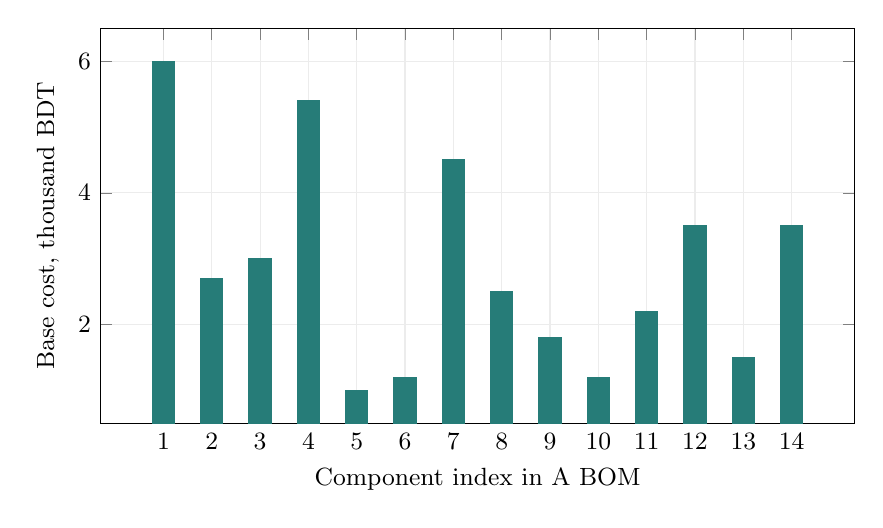
\begin{tikzpicture}\begin{axis}[width=.92\linewidth,height=6.6cm,ylabel={Base cost, thousand BDT},xlabel={Component index in A BOM},xtick=data,bar width=8pt]
\addplot[ybar,fill=teal,draw=teal] coordinates {(1.00000000,6.00000000) (2.00000000,2.70000000) (3.00000000,3.00000000) (4.00000000,5.40000000) (5.00000000,1.00000000) (6.00000000,1.20000000) (7.00000000,4.50000000) (8.00000000,2.50000000) (9.00000000,1.80000000) (10.00000000,1.20000000) (11.00000000,2.20000000) (12.00000000,3.50000000) (13.00000000,1.50000000) (14.00000000,3.50000000)};
\end{axis}\end{tikzpicture}\caption{Base A cost breakdown [D] from [A] component allowances. Indices follow the BOM order; custom rotor, structure and safety costs matter alongside gears.}\end{figure}
\clearpage\section{Sustainable fabrication and build-versus-assemble}
A low-cost process should preserve predictable failure behaviour and repair access. Print patterns and noncritical covers; fabricate balanced rotor sections and structural steel locally; purchase matched bearings and rated drive parts. Recycled aluminium needs traceable alloy and fatigue checks. Recovered HDPE requires contamination and leak inspection. Bamboo is a replaceable noncritical jig/support candidate rather than an assumed structural roof anchor. Material choices require field tests, and neither PLA nor PETG is assumed to harmlessly degrade in a pond. \cite{materials,asa,recycle,khk}

{\small
\setlength{\tabcolsep}{3pt}\renewcommand{\arraystretch}{1.18}
\begin{longtable}{@{}>{\raggedright\arraybackslash}p{0.3193\linewidth}>{\raggedright\arraybackslash}p{0.1996\linewidth}>{\raggedright\arraybackslash}p{0.2714\linewidth}>{\raggedright\arraybackslash}p{0.1197\linewidth}@{}}
\toprule \textbf{Method / process} & \textbf{Low / base / high BDT} & \textbf{Tooling / boundary} & \textbf{Basis} \\ \midrule
\endfirsthead\toprule \textbf{Method / process} & \textbf{Low / base / high BDT} & \textbf{Tooling / boundary} & \textbf{Basis} \\ \midrule
\endhead\bottomrule\endfoot
Printed pattern + formed recycled aluminium rotor. Print segmented pattern, roll/form sheet, rivet, balance & \num{3000} / \num{6000} / \num{11000} & Shared jigs; alloy and fatigue evidence required & [A] Alternative process budgets; overlap BOM \\
Purchased gears / local steel shaft and frame. Machine/key shaft, weld and coat frame, align purchased bearings & \num{5000} / \num{10000} / \num{19000} & Lathe, welding, alignment jig; paid labour and scrap & [A] Alternative process budgets; overlap BOM \\
Recycled PLA / PETG noncritical parts per unit. Dry, filter, print coupons then ducts/covers only & \num{800} / \num{1800} / \num{3500} & Reuse existing printer; no critical strength inferred & [A] Alternative process budgets; overlap BOM \\
Reclaimed HDPE float pair. Inspect contamination, leak-test compartments, mechanically cradle & \num{2400} / \num{4400} / \num{8000} & No toxic drums, no glued untested seams & [A] Alternative process budgets; overlap BOM \\
Bamboo replaceable noncritical fixtures. Dry, treat appropriately, bolt and inspect for rot & \num{500} / \num{1500} / \num{3000} & No untested roof anchor substitution & [A] Alternative process budgets; overlap BOM \\
Recovered metal and polymer take-back per unit. Label material, separate fasteners, recover at end of life & \num{300} / \num{700} / \num{1500} & Recovery target, recycler agreement NOT FOUND & [A] Alternative process budgets; overlap BOM \\
\end{longtable}}
Recycled-polymer research found altered properties and greater variability after reprocessing. It supports coupon testing rather than a blanket claim of equal lifetime. Supplier material guidance supports screening for outdoor UV/temperature suitability; it is not structural qualification for this application. These sources are foreign, and the recycling paper exceeds the age threshold. \cite{recycle,materials,asa}

\subsection{Batch economics}
Per-unit cost is $C(q)=V+F/q$ and the crossover is $q^*=\lceil(F_{make}-F_{assemble})/(V_{assemble}-V_{make})\rceil$. Here ``make means locally fabricate the custom rotor/frame while still buying precision drive elements. Making bearing balls or cutting all gears in-house is not assumed economical. Setup, variable savings, scale capability and rejects are assumptions; crossover is not a sales forecast.

{\small
\setlength{\tabcolsep}{3pt}\renewcommand{\arraystretch}{1.18}
\begin{longtable}{@{}>{\raggedright\arraybackslash}p{0.0666\linewidth}>{\raggedright\arraybackslash}p{0.1110\linewidth}>{\raggedright\arraybackslash}p{0.1998\linewidth}>{\raggedright\arraybackslash}p{0.1998\linewidth}>{\raggedright\arraybackslash}p{0.3329\linewidth}@{}}
\toprule \textbf{Mode} & \textbf{Batch units} & \textbf{Make BDT/unit} & \textbf{Assemble BDT/unit} & \textbf{Crossover / basis} \\ \midrule
\endfirsthead\toprule \textbf{Mode} & \textbf{Batch units} & \textbf{Make BDT/unit} & \textbf{Assemble BDT/unit} & \textbf{Crossover / basis} \\ \midrule
\endhead\bottomrule\endfoot
A & \num{1} & \num{212800} & \num{70000} & \num{21} units; [D] from [A] setup/rates \\
A & \num{10} & \num{50800} & \num{43000} & \num{21} units; [D] from [A] setup/rates \\
A & \num{100} & \num{34600} & \num{40300} & \num{21} units; [D] from [A] setup/rates \\
A & \num{1000} & \num{32980} & \num{40030} & \num{21} units; [D] from [A] setup/rates \\
B & \num{1} & \num{215424} & \num{73200} & \num{20} units; [D] from [A] setup/rates \\
B & \num{10} & \num{53424} & \num{46200} & \num{20} units; [D] from [A] setup/rates \\
B & \num{100} & \num{37224} & \num{43500} & \num{20} units; [D] from [A] setup/rates \\
B & \num{1000} & \num{35604} & \num{43230} & \num{20} units; [D] from [A] setup/rates \\
A+B & \num{1} & \num{428224} & \num{143200} & \num{21} units; [D] from [A] setup/rates \\
A+B & \num{10} & \num{104224} & \num{89200} & \num{21} units; [D] from [A] setup/rates \\
A+B & \num{100} & \num{71824} & \num{83800} & \num{21} units; [D] from [A] setup/rates \\
A+B & \num{1000} & \num{68584} & \num{83260} & \num{21} units; [D] from [A] setup/rates \\
H & \num{1} & \num{364616} & \num{128800} & \num{18} units; [D] from [A] setup/rates \\
H & \num{10} & \num{94616} & \num{83800} & \num{18} units; [D] from [A] setup/rates \\
H & \num{100} & \num{67616} & \num{79300} & \num{18} units; [D] from [A] setup/rates \\
H & \num{1000} & \num{64916} & \num{78850} & \num{18} units; [D] from [A] setup/rates \\
\end{longtable}}
\begin{figure}[htbp]\centering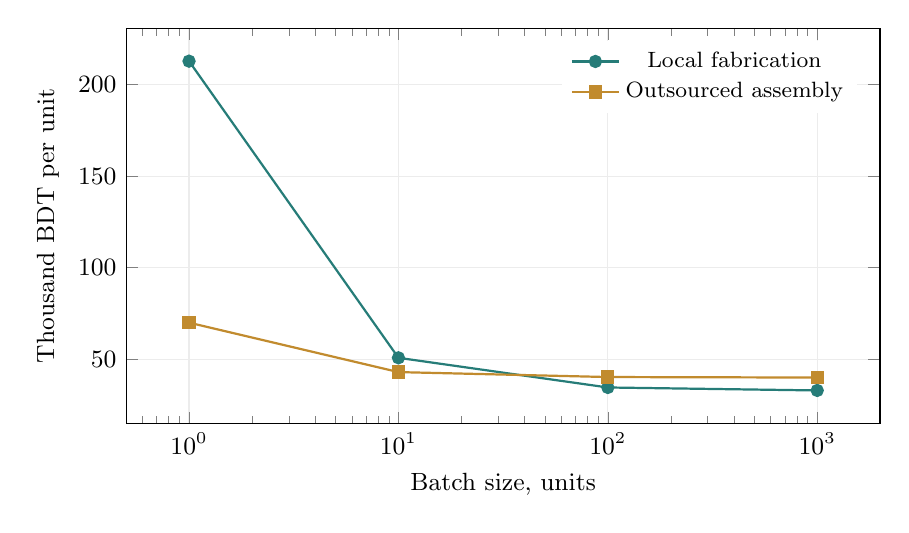
\begin{tikzpicture}\begin{axis}[width=.92\linewidth,height=6.6cm,xmode=log,log basis x=10,xlabel={Batch size, units},ylabel={Thousand BDT per unit},legend pos=north east]
\addplot[teal,thick,mark=*] coordinates {(1.00000000,212.80000000) (10.00000000,50.80000000) (100.00000000,34.60000000) (1000.00000000,32.98000000)};
\addlegendentry{Local fabrication}
\addplot[gold,thick,mark=square*] coordinates {(1.00000000,70.00000000) (10.00000000,43.00000000) (100.00000000,40.30000000) (1000.00000000,40.03000000)};
\addlegendentry{Outsourced assembly}
\end{axis}\end{tikzpicture}\caption{Build versus assemble for A [D] from [A] setup/variable allowances. Precision parts remain purchased in both options.}\end{figure}
\clearpage\section{Equivalent-service comparison and customer affordability}
The cost test holds the useful service boundary explicit. Basic ventilation supplies \num{300} [A] m$^3$/h of added flow to a \num{150} [A] m$^3$ room for \num{4380} [A] h/year; the conventional fan draw is \num{55} [S] W, but the required pressure-flow duty is unmeasured. The pond example needs \num{0.025} [D] kg O2/h continuously. Electric field SAE \num{1.2} [A] kg/kWh and wind field correction \num{0.5} [A] remain assumptions. \cite{fanweb,faoaer,site}

FAO historical foreign tests show example paddlewheel specific oxygen transfer from \num{0.91} [S] to \num{1.41} [S] kg/kWh under their stated conditions; modern supplier nameplates differ. Neither is a clean substitute for a measured field oxygen-transfer curve. The commercial aerator used as a capex reference is larger than the small example demand; energy is duty-normalised, with mixing and start/stop feasibility unresolved. A smaller conventional unit could be cheaper, further weakening the wind case. \cite{faoaer,aerator1,banglaaer}

Wind-only systems have an unmet-service fraction. Equal-service costs therefore retain the conventional machine for backup and charge wind equipment maintenance and replacements on top. The cost of the existing grid connection is common to both alternatives. These totals assume available backup power; outage resilience still needs a generator/battery dispatch and simultaneous-weather assessment. Wind/PV substitution is not a guaranteed hourly service.

{\small
\setlength{\tabcolsep}{3pt}\renewcommand{\arraystretch}{1.18}
\begin{longtable}{@{}>{\raggedright\arraybackslash}p{0.0724\linewidth}>{\raggedright\arraybackslash}p{0.1861\linewidth}>{\raggedright\arraybackslash}p{0.2068\linewidth}>{\raggedright\arraybackslash}p{0.1861\linewidth}>{\raggedright\arraybackslash}p{0.2585\linewidth}@{}}
\toprule \textbf{Base case} & \textbf{Electric, BDT} & \textbf{Wind + backup, BDT} & \textbf{Diesel-fed, BDT} & \textbf{Basis} \\ \midrule
\endfirsthead\toprule \textbf{Base case} & \textbf{Electric, BDT} & \textbf{Wind + backup, BDT} & \textbf{Diesel-fed, BDT} & \textbf{Basis} \\ \midrule
\endhead\bottomrule\endfoot
A & \num{50002} & \num{106569} & \num{198996} & [D] undiscounted horizon totals from [A/S] \\
H & \num{50002} & \num{211770} & \num{198996} & [D] undiscounted horizon totals from [A/S] \\
B & \num{153032} & \num{236983} & \num{285300} & [D] undiscounted horizon totals from [A/S] \\
\end{longtable}}
The verified commercial flat tariff is \num{15.36} [S] BDT/kWh and clinic LT-D1 is \num{9.05} [S] BDT/kWh under the June revision. The scanned official order and correction were inspected visually. Future tariffs are not forecast. VAT and fixed demand charges are not credited as avoidable energy savings on an existing connection. \cite{tarifforder,tariffpage}

\begin{figure}[htbp]\centering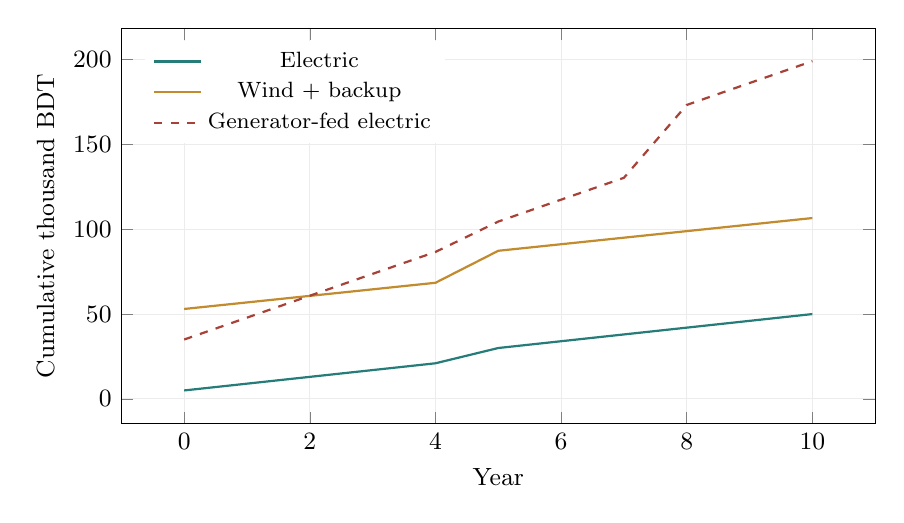
\begin{tikzpicture}\begin{axis}[width=.92\linewidth,height=6.6cm,xlabel={Year},ylabel={Cumulative thousand BDT},legend pos=north west]
\addplot[teal,thick] coordinates {(0.00000000,5.00000000) (1.00000000,9.00022400) (2.00000000,13.00044800) (3.00000000,17.00067200) (4.00000000,21.00089600) (5.00000000,30.00112000) (6.00000000,34.00134400) (7.00000000,38.00156800) (8.00000000,42.00179200) (9.00000000,46.00201600) (10.00000000,50.00224000)};
\addlegendentry{Electric}
\addplot[gold,thick] coordinates {(0.00000000,53.00000000) (1.00000000,56.85685811) (2.00000000,60.71371623) (3.00000000,64.57057434) (4.00000000,68.42743246) (5.00000000,87.28429057) (6.00000000,91.14114869) (7.00000000,94.99800680) (8.00000000,98.85486491) (9.00000000,102.71172303) (10.00000000,106.56858114)};
\addlegendentry{Wind + backup}
\addplot[red,dashed,thick] coordinates {(0.00000000,35.00000000) (1.00000000,47.89960000) (2.00000000,60.79920000) (3.00000000,73.69880000) (4.00000000,86.59840000) (5.00000000,104.49800000) (6.00000000,117.39760000) (7.00000000,130.29720000) (8.00000000,173.19680000) (9.00000000,186.09640000) (10.00000000,198.99600000)};
\addlegendentry{Generator-fed electric}
\end{axis}\end{tikzpicture}\caption{Equal-service cumulative ventilation cost [D] using [A/S] inputs. Generator sharing/fuel assumptions are weak; wind operation alone has unmet demand.}\end{figure}
\subsection{Basic A versus advanced H, and ventilation versus aeration}
{\small
\setlength{\tabcolsep}{3pt}\renewcommand{\arraystretch}{1.18}
\begin{longtable}{@{}>{\raggedright\arraybackslash}p{0.1502\linewidth}>{\raggedright\arraybackslash}p{0.2385\linewidth}>{\raggedright\arraybackslash}p{0.2385\linewidth}>{\raggedright\arraybackslash}p{0.2827\linewidth}@{}}
\toprule \textbf{Criterion} & \textbf{Basic A} & \textbf{Advanced H} & \textbf{Pond B / basis} \\ \midrule
\endfirsthead\toprule \textbf{Criterion} & \textbf{Basic A} & \textbf{Advanced H} & \textbf{Pond B / basis} \\ \midrule
\endhead\bottomrule\endfoot
Principal service & Room air exchange & Wind/PV/battery room air exchange & Supplemental oxygen/mixing; [S/A] concepts \\
Failure during calm & Fan backup required & Limited battery; backup still required & Dangerous pre-dawn DO gap; [A] risk \\
Environmental controls & Intake pollution, rain and pressure & Electrical protection and battery replacement & Corrosion, leaks, mooring, aquatic fragments; [A] \\
Market entry & Supervised noncritical test room & More capital and service skills & Noncritical ornamental pond before stocked aquaculture; [A] judgement \\
Health/yield value & Not monetised & Not monetised & Not monetised; measurements NOT FOUND \\
Wind dependency & Rooftop turbulence & Solar can assist subject to weather/storage & Pond-height shelter and correlated night lulls; [A] \\
\end{longtable}}
{\small
\setlength{\tabcolsep}{3pt}\renewcommand{\arraystretch}{1.18}
\begin{longtable}{@{}>{\raggedright\arraybackslash}p{0.0631\linewidth}>{\raggedright\arraybackslash}p{0.1351\linewidth}>{\raggedright\arraybackslash}p{0.2252\linewidth}>{\raggedright\arraybackslash}p{0.2162\linewidth}>{\raggedright\arraybackslash}p{0.2703\linewidth}@{}}
\toprule \textbf{Case} & \textbf{Wind energy fraction} & \textbf{Annual net energy saving, BDT} & \textbf{Incremental payback} & \textbf{Basis} \\ \midrule
\endfirsthead\toprule \textbf{Case} & \textbf{Wind energy fraction} & \textbf{Annual net energy saving, BDT} & \textbf{Incremental payback} & \textbf{Basis} \\ \midrule
\endhead\bottomrule\endfoot
A & \num{47.1}\% & \num{143.4} & \num{334.8} & [D] after wind maintenance, before health/yield value \\
H & \num{85.0}\% & \num{-6.8} & No finite / beyond decision horizon & [D] after wind maintenance, before health/yield value \\
B & \num{7.6}\% & \num{-1515.1} & No finite / beyond decision horizon & [D] after wind maintenance, before health/yield value \\
\end{longtable}}
{\small
\setlength{\tabcolsep}{3pt}\renewcommand{\arraystretch}{1.18}
\begin{longtable}{@{}>{\raggedright\arraybackslash}p{0.3343\linewidth}>{\raggedright\arraybackslash}p{0.1486\linewidth}>{\raggedright\arraybackslash}p{0.1486\linewidth}>{\raggedright\arraybackslash}p{0.2786\linewidth}@{}}
\toprule \textbf{Case / denominator} & \textbf{Electric cost} & \textbf{Wind + backup cost} & \textbf{Basis} \\ \midrule
\endfirsthead\toprule \textbf{Case / denominator} & \textbf{Electric cost} & \textbf{Wind + backup cost} & \textbf{Basis} \\ \midrule
\endhead\bottomrule\endfoot
A / BDT per added ACH-hour & \num{0.571} & \num{1.217} & [D] total cost / total service, same room volume or oxygen demand \\
H / BDT per added ACH-hour & \num{0.571} & \num{2.417} & [D] total cost / total service, same room volume or oxygen demand \\
B / BDT per field kg O2 & \num{69.878} & \num{108.212} & [D] total cost / total service, same room volume or oxygen demand \\
\end{longtable}}
This is an unsubsidised customer comparison. The additional-flow target is not a full clinic safety specification. Producer profit can coexist with poor customer economics if tariffs are set above avoided energy cost; the report does not call that affordability. Subsidies or sponsor purchases may fund demonstration value, but are not evidence of a sustainable mass-market saving.

\clearpage\section{Wind resource, performance availability and market boundary}
The national NREL campaign establishes a credible measurement/model framework, not a power curve for this prototype. The EU study indexed appendix reports Chandpur at \num{4.11} [S] m/s at \num{60} [S] m, based on the older campaign. Full access to that PDF was blocked, so this contextual number is low-confidence and not used as a rooftop input. Roof turbulence and pond-height shelter need local measurement. \cite{windrepo,euwind,windguide}

The screening uses a Weibull wind distribution with shape $k=2$ [A], $c=\overline v/\Gamma(1+1/k)$ [D], an assumed cut-in and a real-operation cut-out absent from the display model. Numerical integration evaluates both the probability of meeting required shaft power and $E[\min(P_s/P_{needed},1)]$. Mechanical availability multiplies both. A capacity factor relative to the displayed rating is a separate quantity. These are illustrative scenario integrals, not bankable wind-resource forecasts.

{\small
\setlength{\tabcolsep}{3pt}\renewcommand{\arraystretch}{1.18}
\begin{longtable}{@{}>{\raggedright\arraybackslash}p{0.1628\linewidth}>{\raggedright\arraybackslash}p{0.1054\linewidth}>{\raggedright\arraybackslash}p{0.1245\linewidth}>{\raggedright\arraybackslash}p{0.1245\linewidth}>{\raggedright\arraybackslash}p{0.1054\linewidth}>{\raggedright\arraybackslash}p{0.2874\linewidth}@{}}
\toprule \textbf{Scenario} & \textbf{Mean wind m/s} & \textbf{Full service time} & \textbf{Energy fraction} & \textbf{Rated CF} & \textbf{Basis} \\ \midrule
\endfirsthead\toprule \textbf{Scenario} & \textbf{Mean wind m/s} & \textbf{Full service time} & \textbf{Energy fraction} & \textbf{Rated CF} & \textbf{Basis} \\ \midrule
\endhead\bottomrule\endfoot
conservative & \num{2.5} & \num{8.8}\% & \num{24.1}\% & \num{0.6}\% & [D] from [A] distribution, coefficients and uptime \\
base & \num{3.5} & \num{29.2}\% & \num{47.1}\% & \num{1.9}\% & [D] from [A] distribution, coefficients and uptime \\
optimistic & \num{4.5} & \num{48.1}\% & \num{63.6}\% & \num{4.3}\% & [D] from [A] distribution, coefficients and uptime \\
\end{longtable}}
The required wind threshold for the airflow example is \num{4.19} [D] m/s under the assumed geometry and losses. The fraction of time real hardware delivers this output remains NOT FOUND. Published high-tower data cannot supply a measured rooftop/pond availability percentage. The simple annual hybrid energy allowance is separate from the website battery simulation and does not prove hourly adequacy.

{\small
\setlength{\tabcolsep}{3pt}\renewcommand{\arraystretch}{1.18}
\begin{longtable}{@{}>{\raggedright\arraybackslash}p{0.4015\linewidth}>{\raggedright\arraybackslash}p{0.2409\linewidth}>{\raggedright\arraybackslash}p{0.2676\linewidth}@{}}
\toprule \textbf{Serviceable-market search funnel} & \textbf{Low / base / high sites} & \textbf{Basis} \\ \midrule
\endfirsthead\toprule \textbf{Serviceable-market search funnel} & \textbf{Low / base / high sites} & \textbf{Basis} \\ \midrule
\endhead\bottomrule\endfoot
Qualified roof sites in first service territory & \num{100} / \num{500} / \num{1500} & [A] No local qualification or willingness-to-pay survey \\
Qualified supplemental pond sites in first territory & \num{50} / \num{250} / \num{1000} & [A] No local qualification or willingness-to-pay survey \\
\end{longtable}}
National fisheries area and pond count are broad context. A qualified site must pass wind, access, safety, maintenance and payment checks. First customers should be a university demonstration facility, a sponsor-funded community test room or a municipal ornamental-pond pilot. No clinical provider, farmer or sponsor has supplied a purchase commitment in this task. Adoption is a scenario, not a percentage inferred from national hectares.

\clearpage\section{Investment, OPEX, revenue and profit}
\subsection{Prototype-to-market investment}
{\small
\setlength{\tabcolsep}{3pt}\renewcommand{\arraystretch}{1.18}
\begin{longtable}{@{}>{\raggedright\arraybackslash}p{0.3161\linewidth}>{\raggedright\arraybackslash}p{0.1245\linewidth}>{\raggedright\arraybackslash}p{0.1245\linewidth}>{\raggedright\arraybackslash}p{0.1245\linewidth}>{\raggedright\arraybackslash}p{0.2203\linewidth}@{}}
\toprule \textbf{Investment item} & \textbf{Low BDT} & \textbf{Base BDT} & \textbf{High BDT} & \textbf{Treatment / basis} \\ \midrule
\endfirsthead\toprule \textbf{Investment item} & \textbf{Low BDT} & \textbf{Base BDT} & \textbf{High BDT} & \textbf{Treatment / basis} \\ \midrule
\endhead\bottomrule\endfoot
Engineering and redesign & \num{250000} & \num{500000} & \num{1000000} & prelaunch; [A] lines, [D] total \\
Tools printer jigs metrology & \num{200000} & \num{450000} & \num{900000} & capex; [A] lines, [D] total \\
Pilot fabrication and failed trials & \num{150000} & \num{300000} & \num{600000} & prelaunch; [A] lines, [D] total \\
Independent performance and structural tests & \num{150000} & \num{350000} & \num{800000} & prelaunch; [A] lines, [D] total \\
Registration legal and launch & \num{50000} & \num{100000} & \num{200000} & prelaunch; [A] lines, [D] total \\
low total incl contingency and working capital & \num{1060000} & -- & -- & D total; [A] lines, [D] total \\
base total incl contingency and working capital & -- & \num{2240000} & -- & D total; [A] lines, [D] total \\
high total incl contingency and working capital & -- & -- & \num{4600000} & D total; [A] lines, [D] total \\
\end{longtable}}
Totals include an explicitly budgeted contingency and working capital. Prelaunch engineering, pilots, tests, legal/launch and contingency are cash outflows at inception; tools are capitalised, working capital is an asset released at the horizon. Post-launch fleet growth and later tool renewal can raise the financing need far above the initial budget. No government grant is included in project FCF.

\subsection{Fixed OPEX, monthly and annual}
{\small
\setlength{\tabcolsep}{3pt}\renewcommand{\arraystretch}{1.18}
\begin{longtable}{@{}>{\raggedright\arraybackslash}p{0.2888\linewidth}>{\raggedright\arraybackslash}p{0.2625\linewidth}>{\raggedright\arraybackslash}p{0.1662\linewidth}>{\raggedright\arraybackslash}p{0.1925\linewidth}@{}}
\toprule \textbf{Item} & \textbf{Low / base / high monthly BDT} & \textbf{Base annual BDT} & \textbf{Basis} \\ \midrule
\endfirsthead\toprule \textbf{Item} & \textbf{Low / base / high monthly BDT} & \textbf{Base annual BDT} & \textbf{Basis} \\ \midrule
\endhead\bottomrule\endfoot
Engineering and founder salaries & \num{40000} / \num{60000} / \num{100000} & \num{720000} & [A] paid resources; no assumption of permanently free labour \\
Technician salary & \num{18000} / \num{25000} / \num{40000} & \num{300000} & [A] paid resources; no assumption of permanently free labour \\
Rent & \num{8000} / \num{12000} / \num{20000} & \num{144000} & [A] paid resources; no assumption of permanently free labour \\
Utilities and workshop energy & \num{2000} / \num{3500} / \num{6000} & \num{42000} & [A] paid resources; no assumption of permanently free labour \\
Logistics and field travel & \num{4000} / \num{8000} / \num{15000} & \num{96000} & [A] paid resources; no assumption of permanently free labour \\
Marketing and customer development & \num{3000} / \num{7000} / \num{14000} & \num{84000} & [A] paid resources; no assumption of permanently free labour \\
Administration accounting telecom & \num{3000} / \num{6000} / \num{10000} & \num{72000} & [A] paid resources; no assumption of permanently free labour \\
Insurance and liability allowance & \num{1000} / \num{3000} / \num{8000} & \num{36000} & [A] paid resources; no assumption of permanently free labour \\
Tool maintenance and calibration & \num{2000} / \num{4000} / \num{8000} & \num{48000} & [A] paid resources; no assumption of permanently free labour \\
\end{longtable}}
Manufacturing direct cost, sold-unit installation, warranty reserve, provider-fleet service and maintenance-contract delivery are variable costs outside this fixed pool. The base fixed pool escalates with costs and adds a capacity allowance as the calendar ramp grows. Extra headcount required for very high break-even volumes is not validated. Insurance, roof liability and audited tax treatment require quotations/advice. Tax is an explicit profit reserve, with no refund for losses.

\subsection{Proposed commercial models and tariffs}
No sale, lease, pay-per-use, installation or maintenance business model was found in the supplied PDFs or current source. The following are analyst-proposed models requested for appraisal. Competitor prices anchor the opportunity cost but do not substantiate ZeroWatt willingness to pay. \cite{project,poster,site,fanweb,aerator1}

{\small
\setlength{\tabcolsep}{3pt}\renewcommand{\arraystretch}{1.18}
\begin{longtable}{@{}>{\raggedright\arraybackslash}p{0.1487\linewidth}>{\raggedright\arraybackslash}p{0.2450\linewidth}>{\raggedright\arraybackslash}p{0.3937\linewidth}>{\raggedright\arraybackslash}p{0.1225\linewidth}@{}}
\toprule \textbf{Model} & \textbf{Base tariff / transaction} & \textbf{Customer and billing boundary} & \textbf{Basis} \\ \midrule
\endfirsthead\toprule \textbf{Model} & \textbf{Base tariff / transaction} & \textbf{Customer and billing boundary} & \textbf{Basis} \\ \midrule
\endhead\bottomrule\endfoot
Hardware sale & A \num{45000}; B \num{55000}; H \num{125000} BDT & Site owner buys unit; installation unbundled; warranty cost retained & [A] unvalidated WTP \\
Lease & \num{1500} BDT/unit/month & Provider owns fleet; supplemental access, no guaranteed critical service & [A] includes fleet service \\
Pay-per-use & \num{30} BDT/delivered hour & Scheduled \num{120} h/month times wind energy-service fraction; metering/collection untested & [A] provider owns fleet \\
Installation & \num{3000} BDT/sold unit & Separate charge only on sold units; no duplicate leased-asset billing & [A] direct labour allowance \\
Maintenance contract & \num{1800} BDT/year & Eligible sold units after warranty; assumed uptake \num{40}\% & [A] not also billed to lease/use fleet \\
\end{longtable}}
Combined deployments allocate \num{70}\% [A] to sale, \num{20}\% [A] to lease and \num{10}\% [A] to metered use. Product mix is \num{60}\% [A] A, \num{30}\% [A] B and \num{10}\% [A] H. These are mutually exclusive asset channels. Installation and post-warranty service attach only under the stated rules. Assets are not sold and leased simultaneously.

{\small
\setlength{\tabcolsep}{3pt}\renewcommand{\arraystretch}{1.18}
\begin{longtable}{@{}>{\raggedright\arraybackslash}p{0.0758\linewidth}>{\raggedright\arraybackslash}p{0.2085\linewidth}>{\raggedright\arraybackslash}p{0.1706\linewidth}>{\raggedright\arraybackslash}p{0.1706\linewidth}>{\raggedright\arraybackslash}p{0.2844\linewidth}@{}}
\toprule \textbf{Year} & \textbf{New base deployments} & \textbf{Conservative} & \textbf{Optimistic} & \textbf{Basis} \\ \midrule
\endfirsthead\toprule \textbf{Year} & \textbf{New base deployments} & \textbf{Conservative} & \textbf{Optimistic} & \textbf{Basis} \\ \midrule
\endhead\bottomrule\endfoot
\num{1} & \num{30} & \num{15} & \num{54} & [A] ramp; [D] scenario scaling \\
\num{2} & \num{45} & \num{22} & \num{81} & [A] ramp; [D] scenario scaling \\
\num{3} & \num{65} & \num{32} & \num{117} & [A] ramp; [D] scenario scaling \\
\num{4} & \num{90} & \num{45} & \num{162} & [A] ramp; [D] scenario scaling \\
\num{5} & \num{120} & \num{60} & \num{216} & [A] ramp; [D] scenario scaling \\
\num{6} & \num{150} & \num{75} & \num{270} & [A] ramp; [D] scenario scaling \\
\num{7} & \num{180} & \num{90} & \num{324} & [A] ramp; [D] scenario scaling \\
\num{8} & \num{210} & \num{105} & \num{378} & [A] ramp; [D] scenario scaling \\
\num{9} & \num{240} & \num{120} & \num{432} & [A] ramp; [D] scenario scaling \\
\num{10} & \num{270} & \num{135} & \num{486} & [A] ramp; [D] scenario scaling \\
\end{longtable}}
Expected deployments can be fractional in monthly/scenario outputs; actual orders must be integers. New units are spread uniformly across months and are not front-loaded to improve NPV. Cohort churn, collection loss and useful fleet life limit recurring revenue. There is no terminal enterprise multiple or unproven licence revenue.

\subsection{Monthly and annual consolidated results}
{\footnotesize
\setlength{\tabcolsep}{3pt}\renewcommand{\arraystretch}{1.18}
\begin{longtable}{@{}>{\raggedright\arraybackslash}p{0.0569\linewidth}>{\raggedright\arraybackslash}p{0.1706\linewidth}>{\raggedright\arraybackslash}p{0.1706\linewidth}>{\raggedright\arraybackslash}p{0.1479\linewidth}>{\raggedright\arraybackslash}p{0.1251\linewidth}>{\raggedright\arraybackslash}p{0.1706\linewidth}>{\raggedright\arraybackslash}p{0.0683\linewidth}@{}}
\toprule \textbf{Year} & \textbf{Revenue BDT} & \textbf{EBITDA BDT} & \textbf{Depreciation} & \textbf{Tax reserve} & \textbf{Net profit BDT} & \textbf{Basis} \\ \midrule
\endfirsthead\toprule \textbf{Year} & \textbf{Revenue BDT} & \textbf{EBITDA BDT} & \textbf{Depreciation} & \textbf{Tax reserve} & \textbf{Net profit BDT} & \textbf{Basis} \\ \midrule
\endhead\bottomrule\endfoot
\num{0} & \num{0} & \num{-1590000} & \num{0} & \num{0} & \num{-1590000} & [D] \\
\num{1} & \num{1288441} & \num{-1277878} & \num{135474} & \num{0} & \num{-1413352} & [D] \\
\num{2} & \num{2174375} & \num{-1050380} & \num{244891} & \num{0} & \num{-1295272} & [D] \\
\num{3} & \num{3439540} & \num{-690246} & \num{411484} & \num{0} & \num{-1101730} & [D] \\
\num{4} & \num{5145112} & \num{-372399} & \num{655112} & \num{0} & \num{-1027511} & [D] \\
\num{5} & \num{7361558} & \num{132656} & \num{997752} & \num{0} & \num{-865096} & [D] \\
\num{6} & \num{9827825} & \num{747380} & \num{1428463} & \num{0} & \num{-681082} & [D] \\
\num{7} & \num{12532690} & \num{1455905} & \num{1898352} & \num{0} & \num{-442447} & [D] \\
\num{8} & \num{15509036} & \num{2279737} & \num{2442766} & \num{0} & \num{-163029} & [D] \\
\num{9} & \num{18745335} & \num{3202539} & \num{3051453} & \num{37772} & \num{113315} & [D] \\
\num{10} & \num{22228920} & \num{4206666} & \num{3712604} & \num{123515} & \num{370546} & [D] \\
\end{longtable}}
{\footnotesize
\setlength{\tabcolsep}{3pt}\renewcommand{\arraystretch}{1.18}
\begin{longtable}{@{}>{\raggedright\arraybackslash}p{0.0607\linewidth}>{\raggedright\arraybackslash}p{0.1820\linewidth}>{\raggedright\arraybackslash}p{0.1820\linewidth}>{\raggedright\arraybackslash}p{0.1820\linewidth}>{\raggedright\arraybackslash}p{0.1820\linewidth}>{\raggedright\arraybackslash}p{0.1213\linewidth}@{}}
\toprule \textbf{Year} & \textbf{Average monthly revenue} & \textbf{Average monthly EBITDA} & \textbf{Average monthly net profit} & \textbf{Average monthly FCF} & \textbf{Basis} \\ \midrule
\endfirsthead\toprule \textbf{Year} & \textbf{Average monthly revenue} & \textbf{Average monthly EBITDA} & \textbf{Average monthly net profit} & \textbf{Average monthly FCF} & \textbf{Basis} \\ \midrule
\endhead\bottomrule\endfoot
\num{1} & \num{107370} & \num{-106490} & \num{-117779} & \num{-141470} & [D] annual / months \\
\num{2} & \num{181198} & \num{-87532} & \num{-107939} & \num{-148291} & [D] annual / months \\
\num{3} & \num{286628} & \num{-57521} & \num{-91811} & \num{-152644} & [D] annual / months \\
\num{4} & \num{428759} & \num{-31033} & \num{-85626} & \num{-166775} & [D] annual / months \\
\num{5} & \num{613463} & \num{11055} & \num{-72091} & \num{-175590} & [D] annual / months \\
\num{6} & \num{818985} & \num{62282} & \num{-56757} & \num{-220982} & [D] annual / months \\
\num{7} & \num{1044391} & \num{121325} & \num{-36871} & \num{-171801} & [D] annual / months \\
\num{8} & \num{1292420} & \num{189978} & \num{-13586} & \num{-162409} & [D] annual / months \\
\num{9} & \num{1562111} & \num{266878} & \num{9443} & \num{-151906} & [D] annual / months \\
\num{10} & \num{1852410} & \num{350555} & \num{30879} & \num{84070} & [D] annual / months \\
\end{longtable}}
Average monthly rows are annual results divided by operating months; they do not claim every month has equal revenue. The repository includes the full inception-to-horizon monthly schedule for all scenarios, so fleet, working-capital and renewal timing can be inspected.

\subsection{Revenue and profit by model}
{\small
\setlength{\tabcolsep}{3pt}\renewcommand{\arraystretch}{1.18}
\begin{longtable}{@{}>{\raggedright\arraybackslash}p{0.2730\linewidth}>{\raggedright\arraybackslash}p{0.1820\linewidth}>{\raggedright\arraybackslash}p{0.1820\linewidth}>{\raggedright\arraybackslash}p{0.2730\linewidth}@{}}
\toprule \textbf{Year / business model} & \textbf{Annual revenue BDT} & \textbf{Average monthly BDT} & \textbf{Basis} \\ \midrule
\endfirsthead\toprule \textbf{Year / business model} & \textbf{Annual revenue BDT} & \textbf{Average monthly BDT} & \textbf{Basis} \\ \midrule
\endhead\bottomrule\endfoot
1 / sale & \num{1140720} & \num{95060} & [D] from [A] tariffs, cohort and collection inputs \\
1 / lease & \num{55329} & \num{4611} & [D] from [A] tariffs, cohort and collection inputs \\
1 / pay\_per\_use & \num{31282} & \num{2607} & [D] from [A] tariffs, cohort and collection inputs \\
1 / installation & \num{61110} & \num{5092} & [D] from [A] tariffs, cohort and collection inputs \\
1 / maintenance & \num{0} & \num{0} & [D] from [A] tariffs, cohort and collection inputs \\
5 / sale & \num{5337924} & \num{444827} & [D] from [A] tariffs, cohort and collection inputs \\
5 / lease & \num{1053308} & \num{87776} & [D] from [A] tariffs, cohort and collection inputs \\
5 / pay\_per\_use & \num{595521} & \num{49627} & [D] from [A] tariffs, cohort and collection inputs \\
5 / installation & \num{285960} & \num{23830} & [D] from [A] tariffs, cohort and collection inputs \\
5 / maintenance & \num{88844} & \num{7404} & [D] from [A] tariffs, cohort and collection inputs \\
10 / sale & \num{14612402} & \num{1217700} & [D] from [A] tariffs, cohort and collection inputs \\
10 / lease & \num{4107889} & \num{342324} & [D] from [A] tariffs, cohort and collection inputs \\
10 / pay\_per\_use & \num{2322526} & \num{193544} & [D] from [A] tariffs, cohort and collection inputs \\
10 / installation & \num{782807} & \num{65234} & [D] from [A] tariffs, cohort and collection inputs \\
10 / maintenance & \num{403296} & \num{33608} & [D] from [A] tariffs, cohort and collection inputs \\
\end{longtable}}
{\footnotesize
\setlength{\tabcolsep}{3pt}\renewcommand{\arraystretch}{1.18}
\begin{longtable}{@{}>{\raggedright\arraybackslash}p{0.2136\linewidth}>{\raggedright\arraybackslash}p{0.1579\linewidth}>{\raggedright\arraybackslash}p{0.1579\linewidth}>{\raggedright\arraybackslash}p{0.2414\linewidth}>{\raggedright\arraybackslash}p{0.1393\linewidth}@{}}
\toprule \textbf{Year / model} & \textbf{EBITDA annual} & \textbf{Net annual} & \textbf{EBITDA / net monthly} & \textbf{Basis} \\ \midrule
\endfirsthead\toprule \textbf{Year / model} & \textbf{EBITDA annual} & \textbf{Net annual} & \textbf{EBITDA / net monthly} & \textbf{Basis} \\ \midrule
\endhead\bottomrule\endfoot
1 / sale & \num{-1200350} & \num{-1280031} & \num{-100029} / \num{-106669} & [D] allocation below \\
1 / lease & \num{-17993} & \num{-52174} & \num{-1499} / \num{-4348} & [D] allocation below \\
1 / pay\_per\_use & \num{-9708} & \num{-27052} & \num{-809} / \num{-2254} & [D] allocation below \\
1 / installation & \num{-49826} & \num{-54095} & \num{-4152} / \num{-4508} & [D] allocation below \\
1 / maintenance & \num{0} & \num{0} & \num{0} / \num{0} & [D] allocation below \\
5 / sale & \num{-850523} & \num{-915783} & \num{-70877} / \num{-76315} & [D] allocation below \\
5 / lease & \num{598000} & \num{-20046} & \num{49833} / \num{-1670} & [D] allocation below \\
5 / pay\_per\_use & \num{346941} & \num{37076} & \num{28912} / \num{3090} & [D] allocation below \\
5 / installation & \num{22187} & \num{18690} & \num{1849} / \num{1558} & [D] allocation below \\
5 / maintenance & \num{16052} & \num{14966} & \num{1338} / \num{1247} & [D] allocation below \\
10 / sale & \num{-542835} & \num{-696009} & \num{-45236} / \num{-58001} & [D] allocation below \\
10 / lease & \num{2834123} & \num{388992} & \num{236177} / \num{32416} & [D] allocation below \\
10 / pay\_per\_use & \num{1636849} & \num{411468} & \num{136404} / \num{34289} & [D] allocation below \\
10 / installation & \num{156384} & \num{148178} & \num{13032} / \num{12348} & [D] allocation below \\
10 / maintenance & \num{122145} & \num{117917} & \num{10179} / \num{9826} & [D] allocation below \\
\end{longtable}}
Direct costs follow each actual channel. Shared overhead, tools and consolidated tax are allocated by revenue; provider-fleet depreciation follows lease/use deployment shares. These rows reconcile to the combined company but do not prove independent viability of installation or AMC. Separate sale-plus-installation/service, all-lease and all-use alternatives each carry the full overhead and launch budget; they must not be summed.

{\small
\setlength{\tabcolsep}{3pt}\renewcommand{\arraystretch}{1.18}
\begin{longtable}{@{}>{\raggedright\arraybackslash}p{0.2340\linewidth}>{\raggedright\arraybackslash}p{0.1647\linewidth}>{\raggedright\arraybackslash}p{0.1647\linewidth}>{\raggedright\arraybackslash}p{0.1647\linewidth}>{\raggedright\arraybackslash}p{0.1820\linewidth}@{}}
\toprule \textbf{Standalone alternative / year} & \textbf{Annual revenue} & \textbf{Annual EBITDA} & \textbf{Annual net profit} & \textbf{Basis} \\ \midrule
\endfirsthead\toprule \textbf{Standalone alternative / year} & \textbf{Annual revenue} & \textbf{Annual EBITDA} & \textbf{Annual net profit} & \textbf{Basis} \\ \midrule
\endhead\bottomrule\endfoot
sale / 1 & \num{1716900} & \num{-1273188} & \num{-1363188} & [D] full common overhead per alternative \\
sale / 5 & \num{8161041} & \num{-917478} & \num{-1007478} & [D] full common overhead per alternative \\
sale / 10 & \num{22569294} & \num{-315745} & \num{-425244} & [D] full common overhead per alternative \\
lease / 1 & \num{276645} & \num{-1300879} & \num{-1542459} & [D] full common overhead per alternative \\
lease / 5 & \num{5266540} & \num{2353412} & \num{-762429} & [D] full common overhead per alternative \\
lease / 10 & \num{20539447} & \num{13863687} & \num{1307878} & [D] full common overhead per alternative \\
use / 1 & \num{312820} & \num{-1264704} & \num{-1506284} & [D] full common overhead per alternative \\
use / 5 & \num{5955211} & \num{3042083} & \num{-87669} & [D] full common overhead per alternative \\
use / 10 & \num{23225256} & \num{16549497} & \num{3322235} & [D] full common overhead per alternative \\
\end{longtable}}
\begin{figure}[htbp]\centering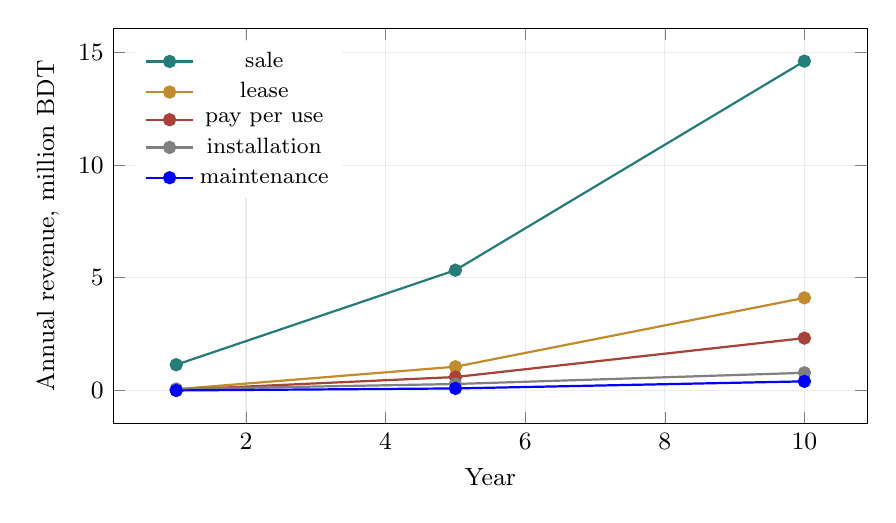
\begin{tikzpicture}\begin{axis}[width=.92\linewidth,height=6.6cm,xlabel={Year},ylabel={Annual revenue, million BDT},legend pos=north west]
\addplot[teal,thick,mark=*] coordinates {(1.00000000,1.14072000) (5.00000000,5.33792423) (10.00000000,14.61240226)};
\addlegendentry{sale}
\addplot[gold,thick,mark=*] coordinates {(1.00000000,0.05532891) (5.00000000,1.05330793) (10.00000000,4.10788931)};
\addlegendentry{lease}
\addplot[red,thick,mark=*] coordinates {(1.00000000,0.03128196) (5.00000000,0.59552106) (10.00000000,2.32252558)};
\addlegendentry{pay per use}
\addplot[gray,thick,mark=*] coordinates {(1.00000000,0.06111000) (5.00000000,0.28596023) (10.00000000,0.78280726)};
\addlegendentry{installation}
\addplot[blue,thick,mark=*] coordinates {(1.00000000,0.00000000) (5.00000000,0.08884424) (10.00000000,0.40329605)};
\addlegendentry{maintenance}
\end{axis}\end{tikzpicture}\caption{Base revenue by proposed model [D] from [A] tariffs and demand. Sales, leases and use have distinct asset cohorts; no double billing.}\end{figure}
\clearpage\section{Cash flow, NPV, IRR and payback}
The model computes $FCF=NetProfit+Depreciation-FleetCapex-ToolCapex-\Delta NWC$ and $NPV=\sum_{m=0}^{M}FCF_m/(1+r)^{m/12}$. The IRR is an annual effective rate solving the same monthly timing equation. Annual summaries are sums of monthly cash flow, not a claim of identical year-end timing. A negative IRR is meaningful when a unique root exists; no root is reported as undefined. Payback is a durable interpolated crossing that subsequent capital outlays do not reverse.

{\footnotesize
\setlength{\tabcolsep}{3pt}\renewcommand{\arraystretch}{1.18}
\begin{longtable}{@{}>{\raggedright\arraybackslash}p{0.1276\linewidth}>{\raggedright\arraybackslash}p{0.2126\linewidth}>{\raggedright\arraybackslash}p{0.1106\linewidth}>{\raggedright\arraybackslash}p{0.2041\linewidth}>{\raggedright\arraybackslash}p{0.1531\linewidth}>{\raggedright\arraybackslash}p{0.1021\linewidth}@{}}
\toprule \textbf{Scenario} & \textbf{NPV BDT / USD} & \textbf{IRR} & \textbf{Simple / discounted payback years} & \textbf{Peak funding BDT} & \textbf{Basis} \\ \midrule
\endfirsthead\toprule \textbf{Scenario} & \textbf{NPV BDT / USD} & \textbf{IRR} & \textbf{Simple / discounted payback years} & \textbf{Peak funding BDT} & \textbf{Basis} \\ \midrule
\endhead\bottomrule\endfoot
conservative & \num{-21129346} / \num{-170880} & Undefined; no root & Not reached / Not reached & \num{49339229} & [D], [A/S] inputs \\
base & \num{-11181078} / \num{-90425} & \num{-47.7}\% & Not reached / Not reached & \num{21769906} & [D], [A/S] inputs \\
optimistic & \num{605233} / \num{4895} & \num{19.6}\% & \num{7.85} / \num{9.96} & \num{6799321} & [D], [A/S] inputs \\
\end{longtable}}
{\small
\setlength{\tabcolsep}{3pt}\renewcommand{\arraystretch}{1.18}
\begin{longtable}{@{}>{\raggedright\arraybackslash}p{0.0858\linewidth}>{\raggedright\arraybackslash}p{0.1717\linewidth}>{\raggedright\arraybackslash}p{0.1717\linewidth}>{\raggedright\arraybackslash}p{0.1717\linewidth}>{\raggedright\arraybackslash}p{0.1975\linewidth}>{\raggedright\arraybackslash}p{0.1116\linewidth}@{}}
\toprule \textbf{Base year} & \textbf{FCF BDT} & \textbf{Fleet capex} & \textbf{Tool capex} & \textbf{Change in working capital} & \textbf{Basis} \\ \midrule
\endfirsthead\toprule \textbf{Base year} & \textbf{FCF BDT} & \textbf{Fleet capex} & \textbf{Tool capex} & \textbf{Change in working capital} & \textbf{Basis} \\ \midrule
\endhead\bottomrule\endfoot
\num{0} & \num{-2240000} & \num{0} & \num{450000} & \num{200000} & [D] monthly sum \\
\num{1} & \num{-1697638} & \num{419760} & \num{0} & \num{0} & [D] monthly sum \\
\num{2} & \num{-1779494} & \num{654826} & \num{0} & \num{74288} & [D] monthly sum \\
\num{3} & \num{-1831730} & \num{983694} & \num{0} & \num{157790} & [D] monthly sum \\
\num{4} & \num{-2001297} & \num{1416519} & \num{0} & \num{212379} & [D] monthly sum \\
\num{5} & \num{-2107080} & \num{1964239} & \num{0} & \num{275497} & [D] monthly sum \\
\num{6} & \num{-2651787} & \num{2553511} & \num{547494} & \num{298163} & [D] monthly sum \\
\num{7} & \num{-2061613} & \num{3186782} & \num{0} & \num{330736} & [D] monthly sum \\
\num{8} & \num{-1948906} & \num{3866629} & \num{0} & \num{362014} & [D] monthly sum \\
\num{9} & \num{-1822866} & \num{4595764} & \num{0} & \num{391870} & [D] monthly sum \\
\num{10} & \num{1008843} & \num{5377044} & \num{0} & \num{-2302737} & [D] monthly sum \\
\end{longtable}}
\begin{figure}[htbp]\centering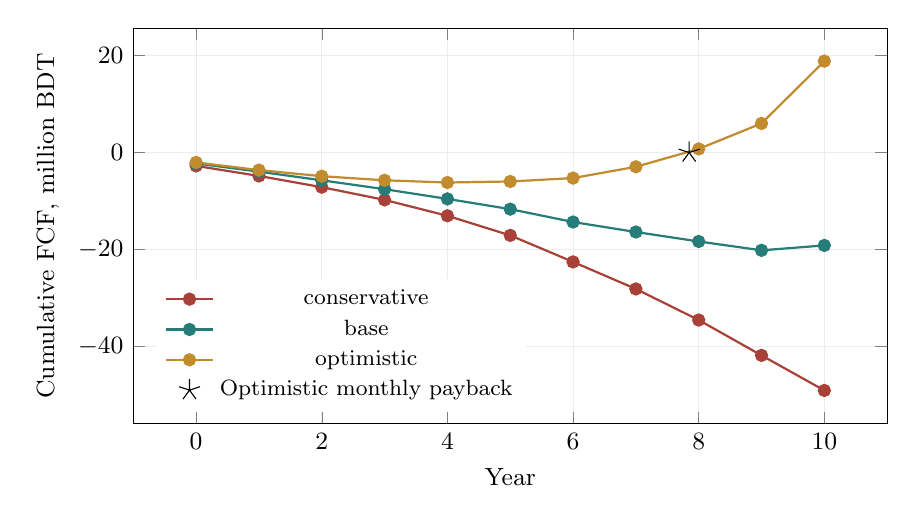
\begin{tikzpicture}\begin{axis}[width=.92\linewidth,height=6.6cm,xlabel={Year},ylabel={Cumulative FCF, million BDT},legend pos=south west]
\addplot[red,thick,mark=*] coordinates {(0.00000000,-2.75000000) (1.00000000,-4.82171202) (2.00000000,-7.13351700) (3.00000000,-9.75434243) (4.00000000,-13.02864607) (5.00000000,-17.06364090) (6.00000000,-22.52912150) (7.00000000,-28.10010796) (8.00000000,-34.50248378) (9.00000000,-41.78555881) (10.00000000,-49.01011636)};
\addlegendentry{conservative}
\addplot[teal,thick,mark=*] coordinates {(0.00000000,-2.24000000) (1.00000000,-3.93763773) (2.00000000,-5.71713148) (3.00000000,-7.54886166) (4.00000000,-9.55015843) (5.00000000,-11.65723851) (6.00000000,-14.30902580) (7.00000000,-16.37063868) (8.00000000,-18.31954449) (9.00000000,-20.14241095) (10.00000000,-19.13356816)};
\addlegendentry{base}
\addplot[gold,thick,mark=*] coordinates {(0.00000000,-2.03600000) (1.00000000,-3.61348543) (2.00000000,-4.87098242) (3.00000000,-5.71636113) (4.00000000,-6.17265483) (5.00000000,-5.95923299) (6.00000000,-5.25676638) (7.00000000,-2.93438515) (8.00000000,0.75114606) (9.00000000,5.99816096) (10.00000000,18.82902081)};
\addlegendentry{optimistic}
\addplot[only marks,mark=star,mark size=4pt,black] coordinates {(7.84791298,0.00000000)};
\addlegendentry{Optimistic monthly payback}
\end{axis}\end{tikzpicture}\caption{Cumulative company cash flow [D]. The star marks optimistic monthly interpolated payback; the base and conservative cases do not recover within the horizon. Lines join annual snapshots.}\end{figure}
\begin{figure}[htbp]\centering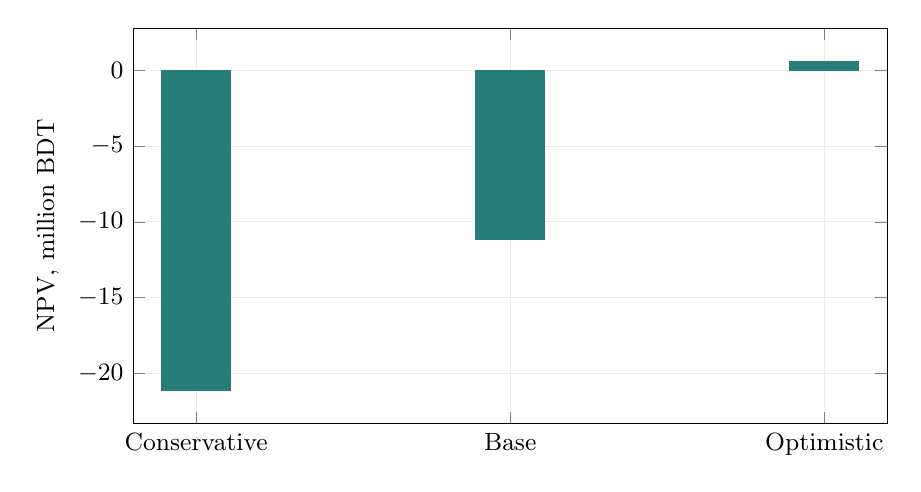
\begin{tikzpicture}\begin{axis}[width=.92\linewidth,height=6.6cm,xtick={1,2,3},xticklabels={Conservative,Base,Optimistic},ylabel={NPV, million BDT},bar width=25pt]
\addplot[ybar,fill=teal,draw=teal] coordinates {(1.00000000,-21.12934584) (2.00000000,-11.18107800) (3.00000000,0.60523275)};
\end{axis}\end{tikzpicture}\caption{Scenario NPV [D] at the assumed base discount rate; positive optimistic results are conditional, not a tuned base forecast.}\end{figure}
{\small
\setlength{\tabcolsep}{3pt}\renewcommand{\arraystretch}{1.18}
\begin{longtable}{@{}>{\raggedright\arraybackslash}p{0.1820\linewidth}>{\raggedright\arraybackslash}p{0.1820\linewidth}>{\raggedright\arraybackslash}p{0.2730\linewidth}>{\raggedright\arraybackslash}p{0.2730\linewidth}@{}}
\toprule \textbf{Scenario} & \textbf{Nominal discount rate} & \textbf{NPV BDT} & \textbf{Basis} \\ \midrule
\endfirsthead\toprule \textbf{Scenario} & \textbf{Nominal discount rate} & \textbf{NPV BDT} & \textbf{Basis} \\ \midrule
\endhead\bottomrule\endfoot
conservative & \num{12}\% & \num{-26789579} & [D] monthly discounting \\
conservative & \num{18}\% & \num{-21129346} & [D] monthly discounting \\
conservative & \num{25}\% & \num{-16757317} & [D] monthly discounting \\
base & \num{12}\% & \num{-13020405} & [D] monthly discounting \\
base & \num{18}\% & \num{-11181078} & [D] monthly discounting \\
base & \num{25}\% & \num{-9622555} & [D] monthly discounting \\
optimistic & \num{12}\% & \num{3733465} & [D] monthly discounting \\
optimistic & \num{18}\% & \num{605233} & [D] monthly discounting \\
optimistic & \num{25}\% & \num{-1463703} & [D] monthly discounting \\
\end{longtable}}
The base and conservative cases fail the required return. The optimistic case assumes more adoption, higher price, cheaper components and stronger wind simultaneously; no probabilities are attached. The initial financing mix below funds only a validation budget and cannot fund the full base-case burn without repeated additional capital. Continuing the base plan would be a financing decision, not evidence that it is feasible.

\clearpage\section{Sensitivity and break-even conditions}
{\small
\setlength{\tabcolsep}{3pt}\renewcommand{\arraystretch}{1.18}
\begin{longtable}{@{}>{\raggedright\arraybackslash}p{0.1786\linewidth}>{\raggedright\arraybackslash}p{0.2211\linewidth}>{\raggedright\arraybackslash}p{0.1701\linewidth}>{\raggedright\arraybackslash}p{0.1701\linewidth}>{\raggedright\arraybackslash}p{0.1701\linewidth}@{}}
\toprule \textbf{Input} & \textbf{Low / high setting} & \textbf{NPV at low} & \textbf{NPV at high} & \textbf{Basis} \\ \midrule
\endfirsthead\toprule \textbf{Input} & \textbf{Low / high setting} & \textbf{NPV at low} & \textbf{NPV at high} & \textbf{Basis} \\ \midrule
\endhead\bottomrule\endfoot
Price & \{'price': 0.8\} / \{'price': 1.2\} & \num{-17524684} & \num{-5821504} & [D] one at a time; [A] ranges \\
Adoption & \{'adoption': 0.6\} / \{'adoption': 1.4\} & \num{-11833030} & \num{-10832513} & [D] one at a time; [A] ranges \\
Wind availability & \{'wind\_factor': 0.6\} / \{'wind\_factor': 1.4\} & \num{-12263177} & \num{-10194117} & [D] one at a time; [A] ranges \\
Component cost & \{'cost': 0.8\} / \{'cost': 1.2\} & \num{-5679524} & \num{-17369983} & [D] one at a time; [A] ranges \\
Discount rate & .12 / .25 & \num{-13020405} & \num{-9622555} & [D] one at a time; [A] ranges \\
\end{longtable}}
\begin{figure}[htbp]\centering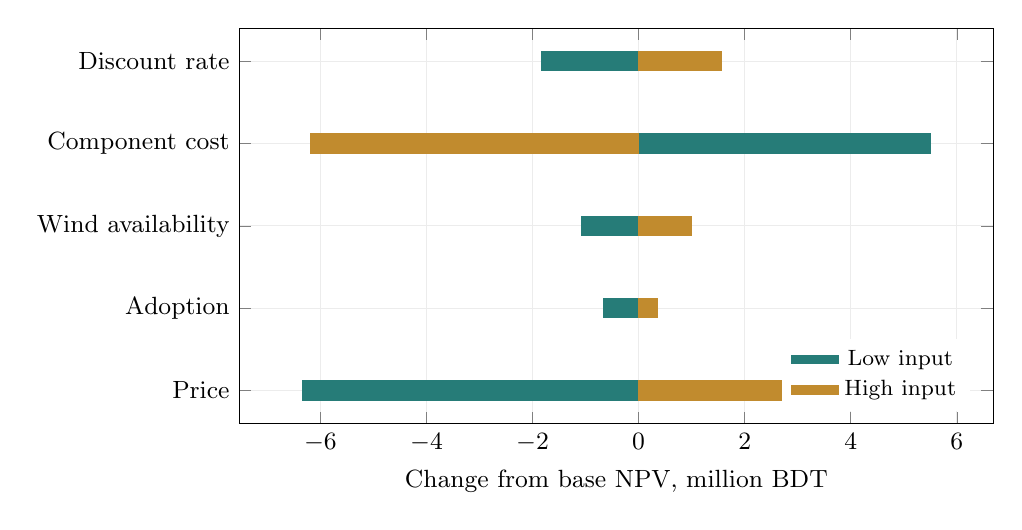
\begin{tikzpicture}\begin{axis}[width=.92\linewidth,height=6.6cm,xlabel={Change from base NPV, million BDT},ytick={1,2,3,4,5},yticklabels={Price,Adoption,Wind availability,Component cost,Discount rate},bar width=7pt,legend pos=south east]
\addplot[xbar,fill=teal,draw=teal] coordinates {(-6.34360585,1.00000000) (-0.65195239,2.00000000) (-1.08209857,3.00000000) (5.50155361,4.00000000) (-1.83932691,5.00000000)};
\addlegendentry{Low input}
\addplot[xbar,fill=gold,draw=gold] coordinates {(5.35957405,1.00000000) (0.34856482,2.00000000) (0.98696134,3.00000000) (-6.18890483,4.00000000) (1.55852301,5.00000000)};
\addlegendentry{High input}
\end{axis}\end{tikzpicture}\caption{Tornado sensitivity [D]. Low/high describe the input, not necessarily the financial outcome. Wind variation affects metered-use hours; sale and supplemental-access lease prices are fixed.}\end{figure}
Within the model, uniformly scaling all tariffs by \num{1.435} [D] makes project NPV zero; the corresponding hardware weighted price is \num{80360} [D] BDT. This is a portfolio tariff condition, not a hardware-only price recommendation. Holding tariff and assumed cost capacity fixed, adoption would need \num{774.17} [D] times the base ramp, including \num{23225.1} [D] expected first-year deployments. That scale is outside the validated staffing/customer envelope and is not a credible sales forecast.

Wind does not directly create sales or guarantee lease uptime in the proposed contracts. Accordingly the financial wind tornado is modest because it changes metered-use revenue only. A severe low-wind reality could also impair adoption, retention, warranty and liability; the one-at-a-time chart does not quantify those interactions. Capacity factor, full-service probability and billable equivalent hours are not used interchangeably.

\clearpage\section{Funding strategy and stage gates}
Pursue non-dilutive pilot support and university facilities first, while keeping project viability separate from fundraising. Government programme amounts are ceilings/indications, not awarded money. No message or application has been sent to any organisation. Probabilities below are subjective low/base/high planning assumptions; published approval probabilities were NOT FOUND.

{\scriptsize
\setlength{\tabcolsep}{3pt}\renewcommand{\arraystretch}{1.18}
\begin{longtable}{@{}>{\raggedright\arraybackslash}p{0.2197\linewidth}>{\raggedright\arraybackslash}p{0.1443\linewidth}>{\raggedright\arraybackslash}p{0.2197\linewidth}>{\raggedright\arraybackslash}p{0.1255\linewidth}>{\raggedright\arraybackslash}p{0.2008\linewidth}@{}}
\toprule \textbf{Route / eligibility} & \textbf{Amount low / base / high BDT} & \textbf{Cost and timing months} & \textbf{Success low / base / high} & \textbf{Basis / limitation} \\ \midrule
\endfirsthead\toprule \textbf{Route / eligibility} & \textbf{Amount low / base / high BDT} & \textbf{Cost and timing months} & \textbf{Success low / base / high} & \textbf{Basis / limitation} \\ \midrule
\endhead\bottomrule\endfoot
University / incubator. University affiliation and supervised test plan & \num{100000} / \num{400000} / \num{700000} & Grant or in-kind, no assumed equity; \num{1} / \num{3} / \num{6} & \num{0}\% / \num{50}\% / \num{80}\% & A; No specific award/call verified \cite{site} \\
CSR / sponsor. Instrumented community benefit and safeguarding agreement & \num{200000} / \num{700000} / \num{1500000} & Restricted pilot grant; reporting and branding; \num{2} / \num{4} / \num{9} & \num{0}\% / \num{25}\% / \num{50}\% & A; Target, not an offer \cite{wb} \\
iDEA / BCC / ICT Division. Confirm innovative hardware eligibility and current application session & \num{200000} / \num{700000} / \num{1000000} & Non-dilutive grant if selected; \num{3} / \num{6} / \num{12} & \num{0}\% / \num{15}\% / \num{30}\% & A/S; S ceiling 1000000, A request/time/chance \cite{idea} \\
Competition. Published call, judged prototype and IP terms & \num{50000} / \num{200000} / \num{500000} & Prize; event-specific rules; \num{1} / \num{4} / \num{12} & \num{0}\% / \num{10}\% / \num{25}\% & A; Current prize amount/deadline NOT FOUND \cite{idea} \\
Angel / impact VC. Paid pilots, unit margin and defensible product & \num{1000000} / \num{3000000} / \num{7000000} & A equity dilution 10-30 percent; no valuation evidence; \num{3} / \num{6} / \num{12} & \num{0}\% / \num{5}\% / \num{15}\% & A; No investor commitment or term sheet \cite{startup} \\
Startup Bangladesh. Registered company, tax/VAT records and diligence & \num{2500000} / \num{5000000} / \num{50000000} & Indexed FAQ: equity/quasi-equity, at most 49 percent; confirm; \num{1} / \num{4} / \num{9} & \num{0}\% / \num{3}\% / \num{10}\% & A/S-index; FAQ indexed terms; full open blocked \cite{startup} \\
SME Foundation. Productive enterprise and participating lender underwriting & \num{50000} / \num{1000000} / \num{1500000} & Published up to 9 percent; current partner terms required; \num{2} / \num{5} / \num{9} & \num{0}\% / \num{10}\% / \num{30}\% & A/S; S indicative amount/interest; A approval time/chance \cite{sme} \\
Bank / BB green refinance. Trade licence, accounts, eligible use and repayment capacity & \num{500000} / \num{1500000} / \num{5000000} & A borrower rate 8-16 percent until current offer; \num{3} / \num{6} / \num{12} & \num{0}\% / \num{5}\% / \num{20}\% & A; Programme exists; product eligibility and rate NOT FOUND \cite{bbcircular} \\
IDCOL. Project sponsor, technical review and eligible financing window & \num{500000} / \num{2000000} / \num{5000000} & Project lending or R\&D route; product-specific offer NOT FOUND; \num{4} / \num{9} / \num{18} & \num{0}\% / \num{3}\% / \num{10}\% & A; Solar terms are not passive-wind eligibility \cite{idcolfees} \\
a2i / ICT innovation. Public service innovation and published eligibility & \num{100000} / \num{500000} / \num{1000000} & Grant, call-specific; \num{3} / \num{6} / \num{12} & \num{0}\% / \num{5}\% / \num{20}\% & A; Current matching call NOT FOUND \cite{idea} \\
GCF / accredited partner. Accredited entity or accepted project-specific route & \num{0} / \num{0} / \num{2000000} & No budgeted receipt; AE/PSAA project route; \num{9} / \num{18} / \num{36} & \num{0}\% / \num{1}\% / \num{5}\% & A; Direct startup allocation NOT FOUND \cite{gcf} \\
BCCRF legacy. Do not assume legacy programme is open & \num{0} / \num{0} / \num{0} & Excluded from recommended cash plan; \num{0} / \num{0} / \num{0} & \num{0}\% / \num{0}\% / \num{0}\% & A; Current actionable call NOT FOUND \cite{wb} \\
Crowdfunding / preorders. Evidence, delivery plan and clear refund terms & \num{100000} / \num{300000} / \num{700000} & A 5-15 percent platform/fulfilment reserve, refunds possible; \num{2} / \num{4} / \num{8} & \num{0}\% / \num{15}\% / \num{35}\% & A; Platform access and legal/FX terms NOT FOUND \cite{site} \\
\end{longtable}}
iDEA criteria and grant cap were checked in its official SOP; the SME route is via participating lenders. The official Bangladesh Bank listing confirms a green-factory refinance circular, but product-specific eligibility, borrower terms and credit approval remain unresolved. Startup Bangladesh FAQ terms are available in indexed text but full-page access failed. IDCOL solar terms must not be transferred to passive mechanical wind, and GCF support generally requires an accredited or accepted project-specific entity route. Current matching BCCRF/a2i/competition calls were NOT FOUND. \cite{idea,sme,bbcircular,startup,idcolfees,gcf}

{\small
\setlength{\tabcolsep}{3pt}\renewcommand{\arraystretch}{1.18}
\begin{longtable}{@{}>{\raggedright\arraybackslash}p{0.2438\linewidth}>{\raggedright\arraybackslash}p{0.1625\linewidth}>{\raggedright\arraybackslash}p{0.1625\linewidth}>{\raggedright\arraybackslash}p{0.1219\linewidth}>{\raggedright\arraybackslash}p{0.2194\linewidth}@{}}
\toprule \textbf{Pilot funding target} & \textbf{BDT} & \textbf{USD} & \textbf{Share} & \textbf{Basis} \\ \midrule
\endfirsthead\toprule \textbf{Pilot funding target} & \textbf{BDT} & \textbf{USD} & \textbf{Share} & \textbf{Basis} \\ \midrule
\endhead\bottomrule\endfoot
Founder cash & \num{440000} & \num{3558} & \num{19.6}\% & [A] none committed \\
University contribution & \num{400000} & \num{3235} & \num{17.9}\% & [A] none committed \\
CSR pilot & \num{700000} & \num{5661} & \num{31.2}\% & [A] none committed \\
iDEA grant target & \num{700000} & \num{5661} & \num{31.2}\% & [A] none committed \\
\end{longtable}}
\begin{figure}[htbp]\centering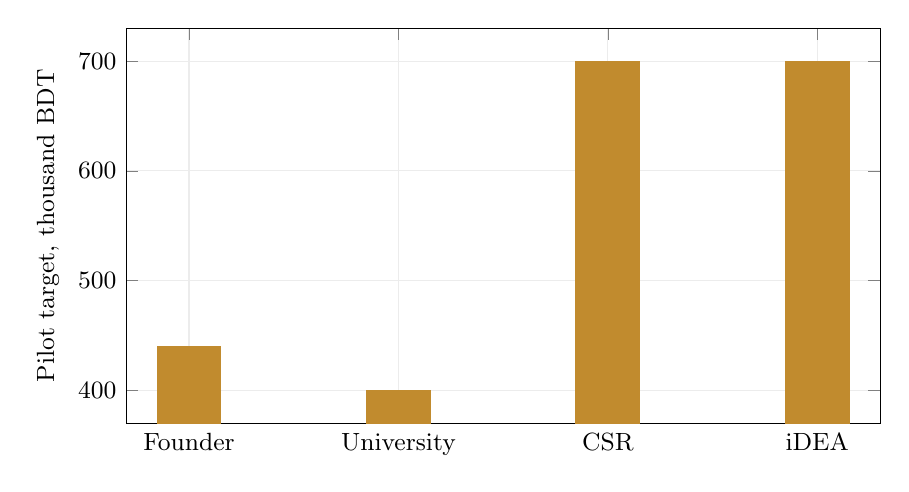
\begin{tikzpicture}\begin{axis}[width=.92\linewidth,height=6.6cm,xtick={1,2,3,4},xticklabels={Founder,University,CSR,iDEA},ylabel={Pilot target, thousand BDT},bar width=23pt]
\addplot[ybar,fill=gold,draw=gold] coordinates {(1.00000000,440.00000000) (2.00000000,400.00000000) (3.00000000,700.00000000) (4.00000000,700.00000000)};
\end{axis}\end{tikzpicture}\caption{Recommended initial funding targets [A], not expected receipts. In-kind contributions offset the relevant budget item, and must not be counted again as unrestricted cash.}\end{figure}
Release funds against gates: first confirm structural safety and a calibrated rotor/load curve; then demonstrate useful airflow or oxygen transfer in supervised conditions; then obtain written customer and supplier commitments. Pause scale spending if a gate fails. Debt should follow evidence of repayment capacity; a lower loan rate cannot turn a structurally negative product value proposition into a sound one.

\clearpage\section{Bangladesh sourcing, assembly and import exposure}
{\small
\setlength{\tabcolsep}{3pt}\renewcommand{\arraystretch}{1.18}
\begin{longtable}{@{}>{\raggedright\arraybackslash}p{0.1756\linewidth}>{\raggedright\arraybackslash}p{0.2874\linewidth}>{\raggedright\arraybackslash}p{0.3193\linewidth}>{\raggedright\arraybackslash}p{0.1277\linewidth}@{}}
\toprule \textbf{Component group} & \textbf{Named source / assembly option} & \textbf{Lead time and landed-cost boundary} & \textbf{Basis} \\ \midrule
\endfirsthead\toprule \textbf{Component group} & \textbf{Named source / assembly option} & \textbf{Lead time and landed-cost boundary} & \textbf{Basis} \\ \midrule
\endhead\bottomrule\endfoot
Patterns and filament & TechShopBD, HTE Bangladesh, Costareen, Electronics.Com.BD & Local stock indication; custom printed work requires quote & [S] observed offers \cite{filament1,filament2,filament3,filament4} \\
Gears and supports & ZerOneTech hobby sample; KHK specification catalogue; Motion/MISUMI bearing references & Production-equivalent matched bores and torque ratings require RFQ & [S/A] not interchangeable \cite{gear,khk,bearing1,bearing2,bearing3} \\
Fan and ducts & Walton distributor for conventional comparator; local sheet-metal workshop RFQ & No verified workshop quote for plenum/roof works & [S/A] \cite{fanweb} \\
Wet hardware / floats & NSC BD and Bangla Ltd. as commercial aerator benchmarks & Complete machines show materials; separate float/paddle supply RFQ needed & [S/A] \cite{aerator1,banglaaer} \\
Custom shafts and frames & Candidate Nawabpur/Dholaikhal workshops; IUT facilities for supervised R\&D & No named, vetted fabricator quote found; do not imply a purchase agreement & [A] sourcing route \\
Imports & Authorised dealer / freight forwarder; NBR classification & Freight, CD, VAT, advance taxes and broker charges depend on exact HS/SRO & [A] exact current duty NOT FOUND \cite{customs} \\
\end{longtable}}
Assumed local lead time is \num{1} [A] / \num{3} [A] / \num{6} [A] weeks; import lead time \num{3} [A] / \num{6} [A] / \num{12} [A] weeks. A landed uplift reserve of \num{15}\% [A] / \num{35}\% [A] / \num{65}\% [A] is only a stress range. It is not a tariff ruling and is not applied again to BOM allowances already intended as domestic purchase budgets. Classified landed quotes are required before procurement.

Assembly acceptance should record rotor balance, shaft alignment, free play, axial retention, brake stop response, guard fasteners, roof water ingress and float leak/stability checks. Keep serialised service records and replaceable wear parts. Production tooling, inspection time and rejected parts are paid costs, not assumed free university support.

\clearpage\section{Future scope with costed evidence gates}
{\footnotesize
\setlength{\tabcolsep}{3pt}\renewcommand{\arraystretch}{1.18}
\begin{longtable}{@{}>{\raggedright\arraybackslash}p{0.3207\linewidth}>{\raggedright\arraybackslash}p{0.1865\linewidth}>{\raggedright\arraybackslash}p{0.1044\linewidth}>{\raggedright\arraybackslash}p{0.2984\linewidth}@{}}
\toprule \textbf{Future item / test} & \textbf{Low / base / high BDT} & \textbf{Timing months} & \textbf{Source and decision boundary} \\ \midrule
\endfirsthead\toprule \textbf{Future item / test} & \textbf{Low / base / high BDT} & \textbf{Timing months} & \textbf{Source and decision boundary} \\ \midrule
\endhead\bottomrule\endfoot
Calibrated performance rig. Torque-speed, static-pressure/flow, DO transfer and brake-stop data & \num{100000} / \num{250000} / \num{500000} & \num{0}--\num{3} & Core validated curves; no revenue booked; [A] budget \cite{windguide,asce,clinic,faoaer} \\
Structural and overspeed redesign. Guard retention, fatigue, anchor uplift and mechanical fail-safe & \num{100000} / \num{250000} / \num{600000} & \num{1}--\num{6} & Independent review before occupied/public installation; [A] budget \cite{windguide,khk} \\
Durable and recycled material pilot. UV, salt exposure, creep, leaks and recycled-lot coupons & \num{50000} / \num{150000} / \num{350000} & \num{2}--\num{6} & Lower lifecycle cost must exceed rework cost; [A] budget \cite{materials,asa,recycle} \\
Monitoring kit per air site. Calibrated CO2, anemometer, RPM and enclosure & \num{7000} / \num{18000} / \num{40000} & \num{3}--\num{6} & Optional electrical load; no measured value premium; [A] budget \cite{whoweb,clinic} \\
Monitoring kit per pond site. DO/temperature logging and reference calibration & \num{12000} / \num{35000} / \num{80000} & \num{3}--\num{6} & Pre-dawn oxygen trend, sensor maintenance required; [A] budget \cite{faoquality,asce} \\
Fixed PV hybrid incremental kit. Matched module, motor, charge control and battery autonomy & \num{20000} / \num{38000} / \num{70000} & \num{6}--\num{12} & Compare fixed PV against costly tracking; no autonomy guarantee; [A] budget \cite{site,windguide} \\
Regional service and modular fleet trial. Multiple independently metered assets and response-time records & \num{100000} / \num{300000} / \num{700000} & \num{9}--\num{18} & Separate additive power from correlated wind availability; [A] budget \cite{faoaer,windguide} \\
Grain grinding feasibility study. Torque requirement, gearing, food-contact and guarding tests & \num{50000} / \num{150000} / \num{300000} & \num{12}--\num{24} & Deferred; not a current business model; [A] budget \cite{project,khk} \\
\end{longtable}}
Each citation supports a method or engineering principle, not an asserted benefit percentage. Spiral-turbine literature concerns other geometries and operating points; no published Cp is copied into a claim about this prototype. Clean-water oxygen-transfer standards and FAO oxygen budgets support testing, while clinic/WHO material supports measurement and intake design. Costs are independent planning alternatives and can overlap the launch test budget; they are not all added to the financial projection. \cite{spiral,spiral2026,asce,faoaer,clinic,whoweb}

\clearpage
\subsection{Roadmap and staged expansion}
The proposed sequence below requires evidence before each expansion step. Test infrastructure, an independent safety review and durability data precede optional monitoring and fleet growth. Costs and dates remain assumptions; an unsuccessful test should delay the next stage rather than trigger automatic deployment.

\begin{figure}[htbp]\centering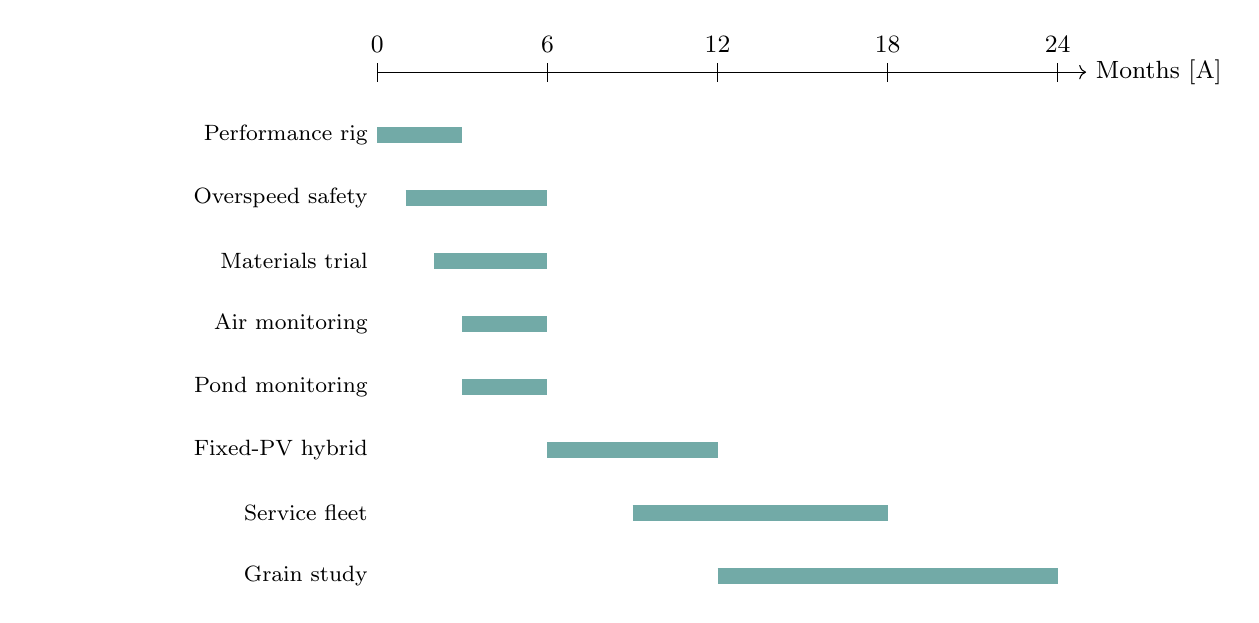
\begin{tikzpicture}[x=.36cm,y=.8cm,font=\small]
\node[anchor=east,text width=42mm,align=right,font=\footnotesize] at (0,0) {Performance rig};
\draw[line width=6pt,teal!65] (0,0)--(3,0);
\node[anchor=east,text width=42mm,align=right,font=\footnotesize] at (0,-1) {Overspeed safety};
\draw[line width=6pt,teal!65] (1,-1)--(6,-1);
\node[anchor=east,text width=42mm,align=right,font=\footnotesize] at (0,-2) {Materials trial};
\draw[line width=6pt,teal!65] (2,-2)--(6,-2);
\node[anchor=east,text width=42mm,align=right,font=\footnotesize] at (0,-3) {Air monitoring};
\draw[line width=6pt,teal!65] (3,-3)--(6,-3);
\node[anchor=east,text width=42mm,align=right,font=\footnotesize] at (0,-4) {Pond monitoring};
\draw[line width=6pt,teal!65] (3,-4)--(6,-4);
\node[anchor=east,text width=42mm,align=right,font=\footnotesize] at (0,-5) {Fixed-PV hybrid};
\draw[line width=6pt,teal!65] (6,-5)--(12,-5);
\node[anchor=east,text width=42mm,align=right,font=\footnotesize] at (0,-6) {Service fleet};
\draw[line width=6pt,teal!65] (9,-6)--(18,-6);
\node[anchor=east,text width=42mm,align=right,font=\footnotesize] at (0,-7) {Grain study};
\draw[line width=6pt,teal!65] (12,-7)--(24,-7);
\draw[->] (0,1)--(25,1) node[right]{Months [A]};\foreach \x in {0,6,12,18,24}{\draw (\x,.85)--(\x,1.15) node[above]{\x};}\end{tikzpicture}\caption{Future-scope sequence [A]. Advancement depends on evidence gates, not elapsed time alone.}\end{figure}
Solar tracking shown in the site adds moving parts; a fixed-panel pilot should establish whether assistance value justifies the extra cost. More pond units add potential transfer but remain exposed to shared lulls. Grain grinding appears only in a submission sketch and remains deferred until torque, food-contact, guarding and economics are tested. No future-feature revenue is included in NPV.

\clearpage\section{Environmental screening and end of life}
The mechanical core uses no operating electricity, but it has embodied materials, fabrication, logistics, lubricant and replacement impacts. A transparent screening calculation is preferable to a zero-carbon claim. The DoE published factor is \num{0.62} [S] kg CO2/kWh for the stated older fiscal periods, published in its January notice. This historical average factor is not a prediction of future marginal displacement or a verified carbon-credit methodology. \cite{gef}

Gross avoided emissions equal displaced grid kWh times the grid factor. Net screening benefit subtracts assumed embodied emissions. Foreground masses are \num{15} [A] kg steel, \num{4} [A] kg aluminium and \num{3} [A] kg polymer for A, or \num{8} [A] kg for B. Assumed factors are \num{2.0} [A], \num{8.0} [A] and \num{3.0} [A] kgCO2e/kg respectively. These are screening placeholders, not supplier EPDs; bounds span half to double the resulting embodied estimate. Hybrid PV/battery/electronics receive an additional lifecycle reserve, not a complete LCA.

{\small
\setlength{\tabcolsep}{3pt}\renewcommand{\arraystretch}{1.18}
\begin{longtable}{@{}>{\raggedright\arraybackslash}p{0.0552\linewidth}>{\raggedright\arraybackslash}p{0.2298\linewidth}>{\raggedright\arraybackslash}p{0.2206\linewidth}>{\raggedright\arraybackslash}p{0.1838\linewidth}>{\raggedright\arraybackslash}p{0.2206\linewidth}@{}}
\toprule \textbf{Case} & \textbf{Embodied low / base / high kgCO2e} & \textbf{Gross avoided over horizon kgCO2} & \textbf{Net screening kgCO2e} & \textbf{Carbon payback years / basis} \\ \midrule
\endfirsthead\toprule \textbf{Case} & \textbf{Embodied low / base / high kgCO2e} & \textbf{Gross avoided over horizon kgCO2} & \textbf{Net screening kgCO2e} & \textbf{Carbon payback years / basis} \\ \midrule
\endhead\bottomrule\endfoot
A & \num{60} / \num{121} / \num{242} & \num{703.7} & \num{582.7} & \num{1.7}; [D], not verified LCA \\
H & \num{210} / \num{421} / \num{842} & \num{1269.5} & \num{848.5} & \num{3.3}; [D], not verified LCA \\
B & \num{68} / \num{136} / \num{272} & \num{85.9} & \num{-50.1} & \num{15.8}; [D], not verified LCA \\
\end{longtable}}
Negative net screening values are retained. Metal recovery is plausible in principle, but no supplier take-back or local recycling recovery rate has been verified. The recovery target in the model is a design target only. Keep material labels, demountable joints, drainable housings and captured lubricants. Recover printed fragments and damaged floats; do not permit pond disposal. Batteries require a dedicated recycler/take-back arrangement.

Noise, structure-borne vibration, wildlife strike/entanglement, corrosion products and aquatic disturbance are NOT MEASURED. Small size and a spiral shape do not prove silence or ecological safety. Use guards and setbacks, survey the site, log vibration/noise at occupied locations, and inspect water impacts. Increasing airflow can introduce outdoor PM and moisture; filtration or damper changes can consume the small pressure budget. \cite{windguide,materials,faoquality}

\clearpage\section{Risks, limitations and decision gates}
{\small
\setlength{\tabcolsep}{3pt}\renewcommand{\arraystretch}{1.18}
\begin{longtable}{@{}>{\raggedright\arraybackslash}p{0.1916\linewidth}>{\raggedright\arraybackslash}p{0.2874\linewidth}>{\raggedright\arraybackslash}p{0.3273\linewidth}>{\raggedright\arraybackslash}p{0.1038\linewidth}@{}}
\toprule \textbf{Risk} & \textbf{Evidence consequence} & \textbf{Action / owner} & \textbf{Basis} \\ \midrule
\endfirsthead\toprule \textbf{Risk} & \textbf{Evidence consequence} & \textbf{Action / owner} & \textbf{Basis} \\ \midrule
\endhead\bottomrule\endfoot
Unknown loaded startup and torque & Core performance cannot be certified & Engineering team: measured torque-speed/load curve before commercial claims & NOT FOUND \\
Wind lulls and site turbulence & Neither time availability nor outage coincidence verified & Independent site assessor: hub-height logging and demand/wind joint analysis & [S/A] \cite{windguide,windrepo} \\
Storm and structural safety & Code rotates in storms; no hardware cut-out proof & Qualified engineer: fatigue, anchorage, guarding and fail-safe test & NOT FOUND \\
Critical clinic / stocked pond liability & Energy example is not safe service delivery & Site owner and expert: define service demand, backup and alarm response & [S/A] \cite{clinic,fao} \\
Custom quotations and warranty & BOM bands may miss costs & Procurement: equivalent-spec written RFQs and pilot failure records & NOT FOUND \\
Demand and tariff acceptance & Proposed revenue may not be realisable & Commercial team: paid pilot, competing offers and customer interviews & NOT FOUND \\
Tax, customs and insurance & Scenario reserves may differ from actual cash outlays & Accountant/broker/insurer: current entity and classification-specific advice & NOT FOUND \\
Future-source access and age & Indexed or dated sources limit confidence & Maintain date/access flags and replace with primary full text & [S] source register \\
\end{longtable}}
Discount-rate sensitivities are not a substitute for modelling correlated failure, supplier escalation or market rejection. The project has no verified production CAD, independent lifetime tests, customer orders or guaranteed grant. All recommendations remain conditional on the explicitly recorded assumptions. A failure to meet an evidence score threshold is reported rather than repaired by raising a self-assigned score.

\clearpage\section{Conclusion}
ZeroWatt Wind is a credible student mechanical concept with an honest poster boundary, but current evidence does not support commercial-scale claims. The base project NPV is \num{-11181078} [D] BDT and its annual effective IRR is \num{-47.7}\% [D]; payback is not reached. The appropriate next investment is a gated measurement and durability pilot. Product redesign, substantially lower cost or independently demonstrated non-energy value would be required before broad rollout. No health, fish-yield, resilience or carbon premium should be promised in advance of evidence.

\clearpage\section{Assumptions and unresolved-evidence register}
{\footnotesize
\setlength{\tabcolsep}{3pt}\renewcommand{\arraystretch}{1.18}
\begin{longtable}{@{}>{\raggedright\arraybackslash}p{0.2505\linewidth}>{\raggedright\arraybackslash}p{0.1085\linewidth}>{\raggedright\arraybackslash}p{0.1085\linewidth}>{\raggedright\arraybackslash}p{0.1085\linewidth}>{\raggedright\arraybackslash}p{0.3339\linewidth}@{}}
\toprule \textbf{Input} & \textbf{Low} & \textbf{Base} & \textbf{High} & \textbf{Basis / reason} \\ \midrule
\endfirsthead\toprule \textbf{Input} & \textbf{Low} & \textbf{Base} & \textbf{High} & \textbf{Basis / reason} \\ \midrule
\endhead\bottomrule\endfoot
FX BDT/USD & \num{123.650} & \num{123.650} & \num{123.650} & S: BB WAR 2026-10-19; not guaranteed transaction rate \\
Site mean wind m/s & \num{2.500} & \num{3.500} & \num{4.500} & A: No hub-height time series; utility-height speeds not transferred to roof \\
Mechanical availability & \num{0.800} & \num{0.900} & \num{0.950} & A: Includes maintenance/curtailment; prototype uptime unmeasured \\
Wind distribution k & \num{1.500} & \num{2.000} & \num{2.500} & A: Only k=2 used in central scenarios; k bounds flagged for later data fitting \\
Price multiplier & \num{0.850} & \num{1.000} & \num{1.100} & A: No willingness-to-pay survey \\
Adoption multiplier & \num{0.500} & \num{1.000} & \num{1.800} & A: No orders or customer funnel \\
Production cost multiplier & \num{0.900} & \num{1.000} & \num{1.250} & A: No comparable RFQs for custom production BOM \\
Annual price/cost escalation & \num{0.020} & \num{0.040} & \num{0.080} & A: Common nominal escalation; no margin inflation benefit \\
Tax reserve fraction & \num{0.200} & \num{0.250} & \num{0.300} & A: Entity-specific statutory taxes NOT FOUND; no tax advice \\
Yearly churn & \num{0.040} & \num{0.080} & \num{0.150} & A: No retention observations \\
Uncollected revenue & \num{0.015} & \num{0.030} & \num{0.080} & A: No payment histories \\
Lease BDT/month & \num{1000.000} & \num{1500.000} & \num{2000.000} & A: Supplemental access tariff; not an energy-saving price quote \\
Pay-per-use BDT/h & \num{20.000} & \num{30.000} & \num{40.000} & A: Metered delivery and collection untested \\
Paid hours scheduled/month & \num{60.000} & \num{120.000} & \num{180.000} & A: Actual billable hours multiplied by energy-service fraction \\
Installation fee BDT & \num{2000.000} & \num{3000.000} & \num{5000.000} & A: Unbundled sold units only \\
AMC fee BDT/year & \num{1000.000} & \num{1800.000} & \num{3000.000} & A: After warranty; separate sold units only \\
Grid benchmark BDT/kWh & \num{9.050} & \num{15.360} & \num{20.000} & A/S: 2026 BERC LT-D1 and LT-E S; future tariff high A; VAT/fixed costs cancel for existing connection \\
Electric field SAE kg/kWh & \num{0.800} & \num{1.200} & \num{1.800} & A: FAO and supplier standard ratings are not field delivery \\
Wind field oxygen correction & \num{0.300} & \num{0.500} & \num{0.700} & A: No alpha/beta or site water test \\
Wind standard SAE kg/kWh & \num{0.400} & \num{0.800} & \num{1.200} & A: Site default base .8, prototype test NOT FOUND \\
Diesel BDT/litre & \num{90.000} & \num{110.000} & \num{140.000} & A: No verified current pump quote \\
Generator litre/kWh & \num{0.300} & \num{0.400} & \num{0.600} & A: Part-load sharing; own set at tiny load could be much worse \\
Embodied footprint multiplier & \num{0.500} & \num{1.000} & \num{2.000} & A: Foreground masses and factors not supplier EPDs \\
Import landed uplift & \num{0.150} & \num{0.350} & \num{0.650} & A: Freight duties and broker reserve; not a statutory tariff \\
Local lead time weeks & \num{1.000} & \num{3.000} & \num{6.000} & A: Custom RFQ not received \\
Import lead time weeks & \num{3.000} & \num{6.000} & \num{12.000} & A: No shipment quote \\
Discount rate nominal & \num{0.120} & \num{0.180} & \num{0.250} & A: Historical 10 percent BB policy benchmark plus project risk; not observed WACC \\
AMC uptake & \num{0.200} & \num{0.400} & \num{0.600} & A: No service-contract demand study \\
Customer mechanical annual maintenance share & \num{0.020} & \num{0.040} & \num{0.080} & A: Service visits can dominate low output \\
Hybrid avoided energy fraction addition & \num{0.250} & \num{0.450} & \num{0.600} & A: Applied to base wind fraction, capped .85; dispatch model NOT FOUND \\
\end{longtable}}
Base assumptions are used as written, not selected to produce a positive outcome. Scenario input combinations are neither statistical confidence intervals nor independent probabilities. Ranges without direct evidence are labelled [A] and should be replaced with measured distributions or written quotations before investment.

{\small
\setlength{\tabcolsep}{3pt}\renewcommand{\arraystretch}{1.18}
\begin{longtable}{@{}>{\raggedright\arraybackslash}p{0.2275\linewidth}>{\raggedright\arraybackslash}p{0.6825\linewidth}@{}}
\toprule \textbf{NOT FOUND / low-confidence item} & \textbf{Required evidence} \\ \midrule
\endfirsthead\toprule \textbf{NOT FOUND / low-confidence item} & \textbf{Required evidence} \\ \midrule
\endhead\bottomrule\endfoot
Measured core performance & Starting wind speed, loaded torque/RPM, Cp, drivetrain loss, airflow/static pressure, field and standard oxygen transfer. \\
Durability and safety & Production stress/fatigue design, safe storm shutdown, anchor/mooring loads, float reserve buoyancy, weathering and service life. \\
Hub-height wind & Bangladesh rooftop/pond distribution, fraction meeting demand, longest lulls and coincidence with outages/pre-dawn DO need. \\
Commercial proof & Current baseline business models/prices in supplied materials, purchase commitments, willingness to pay, retention, collections and market funnel. \\
Component quotations & Three independent comparable production price points for every custom rotor/frame/gear/guard/float/duct and warranted hybrid subsystem. \\
Supplier execution & Verified custom Bangladesh fabricator RFQs, production lead times, landed freight and current HS/SRO tax incidence. \\
Operating/legal costs & Actual insurance, entity-specific tax, minimum/turnover taxes, VAT recoverability, warranty incidence and fleet loss rates. \\
Funding & Programme-specific eligibility, current matching BCCRF/a2i/competition calls, grant success probabilities, committed awards, investor terms and crowdfunding access. \\
Attributable benefits & Local avoided health cost/time, cognitive productivity gain, fish mortality/yield improvement and monetary resilience value. \\
Environmental proof & Supplier EPDs, material masses, recycler recovery rates, audited lifecycle inventory, noise/vibration and wildlife/aquatic impact. \\
Future scope & Measured tracking gain, safe grain-grinding output, validated regional fleet operation and service economics. \\
Blocked source verification & Several official/vendor full texts were blocked or index-only; those records carry explicit access limitations. \\
Gauntlet sufficiency & Evidence-dependent tasks and the financial model may remain below the requested evidence threshold after the maximum rounds; no score is fabricated. \\
\end{longtable}}
\clearpage\section{Gauntlet log summary and reproducibility}
The repository preserves a draft, five task-specific objections and successive source/model repairs for each requested task, plus finance. This is one analyst self-review using investor, judge and fact-checker perspectives; it is not an independent expert review. Evidence sufficiency, arithmetic, realism and completeness are scored separately. Transparent assumptions do not turn an evidence gap into a sourced measurement.

{\footnotesize
\setlength{\tabcolsep}{3pt}\renewcommand{\arraystretch}{1.18}
\begin{longtable}{@{}>{\raggedright\arraybackslash}p{0.0897\linewidth}>{\raggedright\arraybackslash}p{0.0762\linewidth}>{\raggedright\arraybackslash}p{0.2510\linewidth}>{\raggedright\arraybackslash}p{0.4931\linewidth}@{}}
\toprule \textbf{Task} & \textbf{Passes} & \textbf{Scores E / N / R / C} & \textbf{Remaining limitation / Basis} \\ \midrule
\endfirsthead\toprule \textbf{Task} & \textbf{Passes} & \textbf{Scores E / N / R / C} & \textbf{Remaining limitation / Basis} \\ \midrule
\endhead\bottomrule\endfoot
01 & \num{3} & \num{8} / \num{9} / \num{9} / \num{9} & Requested evidence threshold met for bounded description; physical validation still separate. [A] self-assessment \\
02 & \num{6} & \num{6} / \num{9} / \num{9} / \num{9} & NOT FOUND: task-specific field data, comparable quotes or commercial proof; Evidence <8 after maximum rounds. [A] self-assessment \\
03 & \num{6} & \num{7} / \num{9} / \num{9} / \num{9} & NOT FOUND: task-specific field data, comparable quotes or commercial proof; Evidence <8 after maximum rounds. [A] self-assessment \\
04 & \num{6} & \num{6} / \num{10} / \num{9} / \num{9} & NOT FOUND: task-specific field data, comparable quotes or commercial proof; Evidence <8 after maximum rounds. [A] self-assessment \\
05 & \num{6} & \num{6} / \num{10} / \num{9} / \num{9} & NOT FOUND: task-specific field data, comparable quotes or commercial proof; Evidence <8 after maximum rounds. [A] self-assessment \\
06 & \num{6} & \num{6} / \num{10} / \num{9} / \num{9} & NOT FOUND: task-specific field data, comparable quotes or commercial proof; Evidence <8 after maximum rounds. [A] self-assessment \\
07 & \num{6} & \num{6} / \num{10} / \num{9} / \num{9} & NOT FOUND: task-specific field data, comparable quotes or commercial proof; Evidence <8 after maximum rounds. [A] self-assessment \\
08 & \num{6} & \num{5} / \num{10} / \num{9} / \num{9} & NOT FOUND: task-specific field data, comparable quotes or commercial proof; Evidence <8 after maximum rounds. [A] self-assessment \\
09 & \num{6} & \num{6} / \num{10} / \num{9} / \num{9} & NOT FOUND: task-specific field data, comparable quotes or commercial proof; Evidence <8 after maximum rounds. [A] self-assessment \\
10 & \num{6} & \num{7} / \num{9} / \num{9} / \num{9} & NOT FOUND: task-specific field data, comparable quotes or commercial proof; Evidence <8 after maximum rounds. [A] self-assessment \\
11 & \num{6} & \num{7} / \num{9} / \num{9} / \num{9} & NOT FOUND: task-specific field data, comparable quotes or commercial proof; Evidence <8 after maximum rounds. [A] self-assessment \\
12 & \num{3} & \num{9} / \num{10} / \num{9} / \num{9} & Requested evidence threshold met for bounded description; physical validation still separate. [A] self-assessment \\
13 & \num{6} & \num{6} / \num{10} / \num{9} / \num{9} & NOT FOUND: task-specific field data, comparable quotes or commercial proof; Evidence <8 after maximum rounds. [A] self-assessment \\
14 & \num{6} & \num{7} / \num{9} / \num{9} / \num{9} & NOT FOUND: task-specific field data, comparable quotes or commercial proof; Evidence <8 after maximum rounds. [A] self-assessment \\
15 & \num{6} & \num{7} / \num{10} / \num{9} / \num{9} & NOT FOUND: task-specific field data, comparable quotes or commercial proof; Evidence <8 after maximum rounds. [A] self-assessment \\
16 & \num{6} & \num{6} / \num{9} / \num{9} / \num{9} & NOT FOUND: task-specific field data, comparable quotes or commercial proof; Evidence <8 after maximum rounds. [A] self-assessment \\
17 & \num{6} & \num{7} / \num{9} / \num{9} / \num{9} & NOT FOUND: task-specific field data, comparable quotes or commercial proof; Evidence <8 after maximum rounds. [A] self-assessment \\
18 & \num{3} & \num{8} / \num{9} / \num{9} / \num{9} & Requested evidence threshold met for bounded description; physical validation still separate. [A] self-assessment \\
19 & \num{6} & \num{6} / \num{10} / \num{9} / \num{9} & NOT FOUND: task-specific field data, comparable quotes or commercial proof; Evidence <8 after maximum rounds. [A] self-assessment \\
20 & \num{6} & \num{6} / \num{10} / \num{9} / \num{9} & NOT FOUND: task-specific field data, comparable quotes or commercial proof; Evidence <8 after maximum rounds. [A] self-assessment \\
Finance & \num{6} & \num{6} / \num{10} / \num{9} / \num{9} & Unvalidated demand, WTP, resource and production quote inputs; negative base economics retained. [A] self-assessment \\
\end{longtable}}
Reproduction order: run the site audit with Node, run the standard-library Python financial model, then run the report generator. Monetary calculations originate in the model exports; all display rounding and embedded chart data are registered. The standalone TeX uses no external image, bibliography or data file. Source IDs in every citation are checked against the opened-source register. Full monthly/annual tables, assumptions, price observations, BOM, customer comparison, sensitivity and self-check outputs accompany the report.

The financial run passes \num{51} [D] accounting, physical-bound and root-residual self-checks. Compilation and visual QA are documented separately in the repository; arithmetic tests do not validate commercial assumptions.

\clearpage\begin{thebibliography}{99}
\bibitem{aerator1} NSC BD. 4 paddle wheel aerator 2HP. undated. \url{https://nscbd.com/4-paddle-wheel-aerator-2hp-price-in-bangladesh/}. Accessed 2026-10-22. opened content. Bangladesh/project or institutional process. date not established or within 5 years.
\bibitem{asa} Prusa Research. ASA material guidance. undated. \url{https://help.prusa3d.com/article/asa_1809?product=mk4s}. Accessed 2026-10-22. opened content. not Bangladesh-specific. date not established or within 5 years.
\bibitem{asce} ASCE. Measurement of Oxygen Transfer in Clean Water ASCE/EWRI 2-22. 2022. \url{https://ascelibrary.org/doi/book/10.1061/9780784415641}. Accessed 2026-10-22. open attempted; blocked or indexed extract only. not Bangladesh-specific. date not established or within 5 years.
\bibitem{banglaaer} Bangla Ltd.. Aerator machine. undated. \url{https://www.banglaltd.com/product/aerator-machine/}. Accessed 2026-10-22. opened content. Bangladesh. date not established.
\bibitem{battery1} CityTechBD. 12V20Ah LiFePO4 battery pack. undated. \url{https://www.citytechbd.com/12v-20ah-lifepo4-rechargeable-battery-pack}. Accessed 2026-10-22. opened content. Bangladesh/project or institutional process. date not established or within 5 years.
\bibitem{battery2} Teexla. Battery pack category. undated. \url{https://teexla.com/product-category/battery-pack/}. Accessed 2026-10-22. opened content. Bangladesh/project or institutional process. date not established or within 5 years.
\bibitem{bbcircular} Bangladesh Bank. Circular listing. 2026. \url{https://www.bb.org.bd/en/index.php/mediaroom/circular}. Accessed 2026-10-22. opened content. Bangladesh/project or institutional process. date not established or within 5 years.
\bibitem{bdstall} BDStall single seller. SG-PW2-1HP two-paddle aerator. undated. \url{https://www.bdstall.com/details/sg-pw2-1hp-2-paddle-wheel-aerator-for-fish-pond-shrimp-farm-172138/}. Accessed 2026-10-22. opened content. Bangladesh. undated.
\bibitem{bearing1} Daraz / The Fair Enterprise. UCP204 pillow block housed bearing. undated. \url{https://www.daraz.com.bd/products/ucp-204-pillow-block-housed-bearing-i235701366.html}. Accessed 2026-10-22. opened content. Bangladesh/project or institutional process. date not established or within 5 years.
\bibitem{bearing2} MISUMI South East Asia. UCP204 ASAHI SEIKO. undated. \url{https://sg.misumi-ec.com/vona2/detail/221000611249/?HissuCode=UCP204}. Accessed 2026-10-22. open attempted; blocked or indexed extract only. not Bangladesh-specific. date not established or within 5 years.
\bibitem{bearing3} Motion. AMI UCP204. undated. \url{https://www.motion.com/products/sku/00561782}. Accessed 2026-10-22. opened content. not Bangladesh-specific. date not established or within 5 years.
\bibitem{clinic} PLOS Global Public Health / PMC. Direct estimates of absolute ventilation and estimated tuberculosis transmission risk in clinics in South Africa. 2022-11-02. \url{https://pmc.ncbi.nlm.nih.gov/articles/PMC10021606/}. Accessed 2026-10-22. opened content. not Bangladesh-specific. date not established or within 5 years.
\bibitem{cognition} Environmental Research Letters / Cedeno Laurent et al.. Associations between acute PM2.5 and carbon dioxide exposure and cognition. 2021-09-09. \url{https://doi.org/10.1088/1748-9326/ac1bd8}. Accessed 2026-10-22. open attempted; blocked or indexed extract only. not Bangladesh-specific. OLDER THAN 5 YEARS.
\bibitem{customs} National Board of Revenue. Bangladesh Customs tariff portal. 2026. \url{https://customs.gov.bd/index.jsf}. Accessed 2026-10-22. open attempted; blocked or indexed extract only. Bangladesh/project or institutional process. date not established or within 5 years.
\bibitem{dof} Department of Fisheries. Yearbook of Fisheries Statistics Bangladesh 2023-24. 2024-12. \url{https://objectstorage.ap-dcc-gazipur-1.oraclecloud15.com/n/axvjbnqprylg/b/V2Ministry/o/office-fisheries/2024/12/4c64d1e387d446ec97430228bcc06ddc.pdf}. Accessed 2026-10-22. opened content. Bangladesh/project or institutional process. date not established or within 5 years.
\bibitem{euwind} European Union Delegation to Bangladesh. Wind energy study Bangladesh final report. 2022-02. \url{https://www.eeas.europa.eu/sites/default/files/documents/2023/Final%20report%2008022022_wind%20study.pdf}. Accessed 2026-10-22. open attempted; blocked or indexed extract only. Bangladesh/project or institutional process. date not established or within 5 years.
\bibitem{fanweb} Walton. WEF1201N 12 inch exhaust fan. undated. \url{https://waltonbd.com/water-pump/electrical-appliances/fan/exhaust-fan/wef1201n-12}. Accessed 2026-10-22. opened content. Bangladesh/project or institutional process. date not established or within 5 years.
\bibitem{fao} FAO. Manual on polyculture and integrated fish farming in Bangladesh. unknown; legacy. \url{https://www.fao.org/4/AC375E/AC375E05.htm}. Accessed 2026-10-22. opened content. Bangladesh/project or institutional process. OLDER THAN 5 YEARS / legacy underlying evidence.
\bibitem{faoaer} FAO. Aeration and Oxygenation in Aquaculture chapter 21. legacy; underlying trials 1982. \url{https://www.fao.org/4/X5744E/x5744e0m.htm}. Accessed 2026-10-22. opened content. not Bangladesh-specific. OLDER THAN 5 YEARS / legacy underlying evidence.
\bibitem{faoquality} FAO. Improving Pond Water Quality. legacy; date not stated. \url{https://www.fao.org/fishery/static/FAO_Training/FAO_Training/General/x6709e/x6709e02.htm}. Accessed 2026-10-22. opened content. not Bangladesh-specific. OLDER THAN 5 YEARS / legacy underlying evidence.
\bibitem{filament1} Costareen. Filament price guide. 2026-10-01. \url{https://costareen.com/2026/10/01/filament-price-in-bangladesh-guide/}. Accessed 2026-10-22. opened content. Bangladesh/project or institutional process. date not established or within 5 years.
\bibitem{filament2} TechShopBD. Marketplace filament offers. undated. \url{https://techshopbd.com/marketplace}. Accessed 2026-10-22. opened content. Bangladesh/project or institutional process. date not established or within 5 years.
\bibitem{filament3} HTE Bangladesh. PLA filament 1 kg. undated. \url{https://www.htebd.com/3d-printing-filament-pla-1kg/}. Accessed 2026-10-22. opened content. Bangladesh/project or institutional process. date not established or within 5 years.
\bibitem{filament4} Electronics.Com.BD. PLA filament white 1kg. undated. \url{https://electronics.com.bd/pla-3d-printer-filament-1-75mm-1kg2-2lb-white}. Accessed 2026-10-22. opened content. Bangladesh/project or institutional process. date not established or within 5 years.
\bibitem{fx} Bangladesh Bank. Exchange Rate of Taka. 2026-10-19. \url{https://www.bb.org.bd/en/index.php/econdata/exchangerate}. Accessed 2026-10-22. opened content. Bangladesh/project or institutional process. date not established or within 5 years.
\bibitem{gcf} Green Climate Fund. Project Preparation Facility process. 2026. \url{https://www.greenclimate.fund/access-funding/project-preparation-facility/process}. Accessed 2026-10-22. open attempted; blocked or indexed extract only. Bangladesh/project or institutional process. date not established or within 5 years.
\bibitem{gear} ZerOneTech BD. Bevel gear 8mm hole 20 teeth CNA015. undated. \url{https://www.zeronetechbd.com/product/details/bevel-gear-8mm-hole-model-gear-90-degree-transmission-steering-20-teethcna015}. Accessed 2026-10-22. open attempted; blocked or indexed extract only. Bangladesh/project or institutional process. date not established or within 5 years.
\bibitem{gef} Department of Environment. Grid Emission Factor for Bangladesh. 2025-01-23. \url{https://objectstorage.ap-dcc-gazipur-1.oraclecloud15.com/n/axvjbnqprylg/b/V2Ministry/o/office-doe/2024/12/ea2411221c1f4ff49805bb7ac39c66fa.pdf}. Accessed 2026-10-22. opened content. Bangladesh/project or institutional process. date not established or within 5 years.
\bibitem{harvard} Harvard T.H. Chan School. Office air quality may affect employees cognition productivity. 2021-09-09. \url{https://hsph.harvard.edu/news/office-air-quality-may-affect-employees-cognition-productivity/}. Accessed 2026-10-22. opened content. not Bangladesh-specific. OLDER THAN 5 YEARS.
\bibitem{heatnews} Bangladesh Sangbad Sangstha. Scorching heat wave affecting aquatic species livestock. 2024. \url{https://www.bssnews.net/news/184834}. Accessed 2026-10-22. opened content. Bangladesh/project or institutional process. date not established or within 5 years.
\bibitem{idcolfees} IDCOL. Fees and charges. undated. \url{https://www.idcol.org/idcol_new/public/fees-charge}. Accessed 2026-10-22. opened content. Bangladesh/project or institutional process. date not established or within 5 years.
\bibitem{idea} iDEA / Bangladesh Computer Council. Selection procedures for pre-seed grant. undated. \url{https://apply.idea.gov.bd/SOP.pdf}. Accessed 2026-10-22. opened content. Bangladesh/project or institutional process. date not established or within 5 years.
\bibitem{khk} KHK Gears. Bevel gears catalogue. 2025. \url{https://khkgears.net/pdf/2025/bevel-gears.pdf}. Accessed 2026-10-22. opened content. not Bangladesh-specific. within 5 years.
\bibitem{materials} Prusa Research. Filament Material Guide. undated. \url{https://help.prusa3d.com/filament-material-guide}. Accessed 2026-10-22. opened content. not Bangladesh-specific. date not established or within 5 years.
\bibitem{poster} Project team. ZeroWatt Wind poster. 2026; undated. \url{file:///G:/new_8/zerowatt-wind-v8/inputs/poster.pdf}. Accessed 2026-10-22. opened content. Bangladesh/project or institutional process. date not established or within 5 years.
\bibitem{project} Project team. ZeroWatt Wind CezeriFest submission. 2026-09-15. \url{file:///G:/new_8/zerowatt-wind-v8/inputs/project.pdf}. Accessed 2026-10-22. opened content. Bangladesh/project or institutional process. date not established or within 5 years.
\bibitem{rate} Bangladesh Bank. Monetary Policy Review FY2024-25. 2025. \url{https://www.bb.org.bd/pub/halfyearly/monetaryprev/mpr_2024_25.pdf}. Accessed 2026-10-22. opened content. Bangladesh/project or institutional process. date not established or within 5 years.
\bibitem{recycle} 3D Printing and Additive Manufacturing / Anderson. Mechanical Properties of Specimens 3D Printed with Virgin and Recycled Polylactic Acid. 2017. \url{https://journals.sagepub.com/doi/10.1089/3dp.2016.0054}. Accessed 2026-10-22. opened content. not Bangladesh-specific. OLDER THAN 5 YEARS.
\bibitem{site} Project repository. ZeroWatt simulation engineering source audit. 2026-10-22 audit. \url{file:///G:/new_8/zerowatt-wind-v8/data/site_baseline.json}. Accessed 2026-10-22. opened content. Bangladesh/project or institutional process. date not established or within 5 years.
\bibitem{sme} SME Foundation. Credit wholesaling programme. undated. \url{https://wehelp.smef.gov.bd/blog-details/credit-wholeshelling}. Accessed 2026-10-22. opened content. Bangladesh/project or institutional process. date not established or within 5 years.
\bibitem{spiral} Energies / Jang et al.. Analysis of Archimedes Spiral Wind Turbine Performance by Simulation and Field Test. 2019. \url{https://www.mdpi.com/1996-1073/12/24/4624}. Accessed 2026-10-22. open attempted; blocked or indexed extract only. Bangladesh/project or institutional process. OLDER THAN 5 YEARS.
\bibitem{spiral2026} Energy Reports. Design optimization and performance evaluation of a 3D-printed Archimedes Spiral Wind Turbine for renewable energy generation in Bangladesh. 2026-06. \url{https://www.sciencedirect.com/science/article/pii/S2352484726000946}. Accessed 2026-10-22. open attempted; blocked or indexed extract only. Bangladesh/project or institutional process. date not established or within 5 years.
\bibitem{startup} Startup Bangladesh Limited. Frequently asked questions. undated. \url{https://www.startupbangladesh.vc/contact/faqs/}. Accessed 2026-10-22. open attempted; blocked or indexed extract only. Bangladesh/project or institutional process. date not established or within 5 years.
\bibitem{tarifforder} BERC via Power Division. Retail electricity tariff and correction orders. 2026-06-03; correction 2026-06-04. \url{https://objectstorage.ap-dcc-gazipur-1.oraclecloud15.com/n/axvjbnqprylg/b/V2Ministry/o/office-powerdivision/2026/5/73ea43ec-d2a1-4856-a3be-6c6b93e6ae76.pdf}. Accessed 2026-10-22. opened content. Bangladesh/project or institutional process. date not established or within 5 years.
\bibitem{tariffpage} Power Division Bangladesh. Retail electricity rates. 2026-06-09. \url{https://powerdivision.gov.bd/pages/static-pages/694032a035ce18e1c055f992}. Accessed 2026-10-22. opened content. Bangladesh/project or institutional process. date not established or within 5 years.
\bibitem{wb} World Bank. Addressing Environmental Pollution is Critical for Bangladesh Growth and Development. 2024-03-28. \url{https://www.worldbank.org/en/news/press-release/2024/03/28/addressing-environmental-pollution-is-critical-for-bangladesh-s-growth-and-development}. Accessed 2026-10-22. opened content. Bangladesh/project or institutional process. date not established or within 5 years.
\bibitem{whoweb} WHO. Ventilation roadmap publication page. 2021-03-01. \url{https://www.who.int/publications/i/item/9789240021280}. Accessed 2026-10-22. opened content. not Bangladesh-specific. OLDER THAN 5 YEARS.
\bibitem{windguide} US Department of Energy. Small Wind Guidebook. 2025. \url{https://www.energy.gov/cmei/systems/windexchange/small-wind-guidebook}. Accessed 2026-10-22. opened content. not Bangladesh-specific. date not established or within 5 years.
\bibitem{windrepo} NREL / NLR research hub. Assessing the Wind Energy Potential in Bangladesh. 2018. \url{https://research-hub.nlr.gov/en/publications/assessing-the-wind-energy-potential-in-bangladesh-enabling-wind-e/}. Accessed 2026-10-22. opened content. Bangladesh/project or institutional process. OLDER THAN 5 YEARS.
\end{thebibliography}\end{document}
